\documentclass{article}
\usepackage{iclr2027_conference,times}
\usepackage{fontspec}
\setmainfont{texgyretermes}[Extension=.otf, UprightFont=*-regular, BoldFont=*-bold,
  ItalicFont=*-italic, BoldItalicFont=*-bolditalic]
\usepackage{hyperref}
\hypersetup{hidelinks}
\usepackage{url}
\usepackage{graphicx}
\usepackage{booktabs}
\usepackage{array}
\usepackage{longtable}
\usepackage{amsmath}
\usepackage{amssymb}
\usepackage{microtype}
\usepackage{amsthm}
\newcounter{none}
\providecommand{\tightlist}{\setlength{\itemsep}{0pt}\setlength{\parskip}{0pt}}
\newtheorem{proposition}{Proposition}
\title{BrainLLM-Bench:\\
Model Rankings Transfer Across Listeners\\
but Not Always Across Stimuli or Readouts}
% Public-release snapshot of the R1 manuscript source (MEG@9f2a3165) that the checkers in codes/ read.
\author{Xupeng Chen$^{1,*}$ \quad Michael Yue$^{2}$ \quad Runhao Li$^{3}$ \quad Jiayi Cheng$^{1}$ \quad Chenqian Le$^{1}$ \\
{\normalfont $^{1}$New York University \quad $^{2}$Columbia University \quad $^{3}$University of Southern California} \\
{\normalfont $^{*}$Corresponding author: \texttt{xc1490@nyu.edu}}}
\newcommand{\coderepo}{\url{https://github.com/james20141606/BrainLLM-Bench}}
\begin{document}
\maketitle

\begin{abstract}
Reading a brain-likeness leaderboard as a fact about models assumes its ranking survives a
change of readout, listeners or text. On one listener's MEG, $32$ checkpoints get a
reliable leaderboard from representational similarity (ranking reliability $0.98$) and an equally
reliable one from linear encoding ($0.96$), in \emph{opposite} orders ($\rho = -0.573$, family-clustered $95\%$ CI $[-0.79, -0.26]$). Brain-likeness benchmarks usually score with one primary readout and resample
only participants, so they usually do not report this, or whether a ranking survives a change of text.
BrainLLM-Bench changes readout, listeners and stimulus one at a time. Listeners barely move a
leaderboard: disjoint listener halves agree at median Spearman $\rho$ of $+0.764$ to $+0.961$ (two
crossed cohorts, both readouts). The reversal, for the readouts as conventionally applied (masked
models also read the words after the target),
survives the $48$ base checkpoints of the registered test under family-clustered uncertainty ($\rho = -0.59$, CI $[-0.78, -0.12]$) but belongs to one cohort: it does not reproduce on $27$-listener
MEG and is not determined on $47$-subject English EEG once slow drift is removed, and feature geometry is not excluded. On the $32$ checkpoints it is not
determined when the $14$ masked and encoder--decoder checkpoints are read up to the target word, as
the causal ones are ($\rho = -0.016$, CI $[-0.40, +0.34]$), or once static embeddings are also
partialled out ($\rho = -0.415$). Text depends on the cohort:
on four narratives heard by the same $27$ listeners, similarity leaderboards from different stories
do not transfer (mean agreement near zero; exploratory --- the registered co-primary supports it,
the registered dispersion primary did not), while a fully crossed fMRI cohort ($25$ narratives
$\times$ $9$ listeners) transfers well ($+0.778$). The benchmark behind these tests is one protocol
over five language cohorts (MEG, EEG and intracranial ECoG; English and German; scalp EEG an
uncontrolled probe), six leaderboard models and a readout sweep extended from $32$ to $57$
checkpoints ($48$ base) spanning $2019$--$2026$. We prove which feature transformations each
readout ignores; this shows the two can disagree without either being wrong, not that this is why
they disagree here, and the reversal is a disagreement between measurements, not a refutation of
brain-likeness. Model size did not consistently order alignment on a Pythia ladder ($70$M--$2.8$B)
or across three Qwen generations (up to $72$B). A brain-likeness ranking
is a claim about a readout, a cohort and a stimulus sample, and should name all three.
\end{abstract}

\section{Introduction}\label{introduction}

Leaderboards that score language models against brain recordings are used to say which model is
most brain-like and whether larger ones are more so. Score $32$ checkpoints from $12$ families against one
listener's MEG, over twelve sessions of Sherlock Holmes audiobooks. Representational similarity
\citep{kriegeskorte2008representational} returns a leaderboard with ranking reliability $0.98$; ridge encoding
\citep{huth2016natural} returns an equally reliable one ($0.96$). The
two order the checkpoints in opposite directions ($\rho=-0.573$): similarity puts the
autoregressive models last and encoding puts them first.

\begin{figure}[t]
\centering
\includegraphics[width=\textwidth]{../figures_v2/fig1_20261010/fig1.pdf}
\caption{\textbf{A model ranking survives new listeners, but not always a new story or a new readout.} Rows change one argument of Eq.~\eqref{eq:agree}. Dots: listener-half splits or story pairs; bars: medians (Table~\ref{tab:main}). Diamonds: readout concordance, family-clustered 95\% intervals; grey circles: reliability ceiling. With each model's static layer-0 embedding (C4) also partialled out, the reversal is not determined, nor under a common reading rule. $^\dagger$Exploratory. Brennan EEG is omitted: its epochs were not baseline-corrected, and after drift removal its concordance is not determined.}
\label{fig:overview}
\end{figure}

The readout is usually chosen silently: brain-likeness benchmarks score with one primary readout
\citep{schrimpf2020integrative, schrimpf2021neural}, size-scaling results each rest on one
\citep{antonello2024scaling, hong2026larger}, and single alignment numbers are already fragile to
positional and word-rate confounds \citep{feghhi2026spurious} and to trivial baselines
\citep{lai2025illusions}. In vision, which network looks most brain-like already flips with the
similarity measure \citep{soni2024conclusions}. Benchmarks put their error bars over participants, but a reader of
``model $X$ is more brain-like'' assumes the ranking also survives another readout and another
text. Resampling listeners cannot test the second, since every listener heard the same words: the
language-as-fixed-effect fallacy \citep{clark1973language, westfall2016fixing,
yarkoni2020generalizability}, acting on model rankings rather than on effect estimates.

BrainLLM-Bench makes readout, listeners and text explicit axes (Figure~\ref{fig:overview}): it
fixes the protocol (statistic, confound battery, ceiling, null) and changes one argument of a
ranking at a time (Section~\ref{sec:setup}).
Resampling \emph{listeners} (on LibriBrain, sessions) barely moves a leaderboard in all four LibriBrain readout and aggregation
combinations and in both crossed cohorts. The \emph{readout} reversal survives family-clustered inference and the $48$
base checkpoints of the registered test, but not a common reading rule: read up to the target word,
as the causal ones are, the $14$ masked and encoder--decoder checkpoints leave it not determined. Changing the \emph{text} leaves story leaderboards in
place in one crossed cohort and not in the other. What drives the
reversal is outside what these data identify: under the class-specific reading rule $56\%$ of it is a between-class offset;
it does not travel to MEG-MASC (positive, with a family-clustered interval excluding zero narrowly), and on Brennan EEG, once slow drift is removed, it is not determined;
feature geometry is not excluded (standardized-feature similarity leaves a
family-clustered interval crossing zero), and Proposition~\ref{prop:invariance} shows that readouts can
disagree, not why ours do; the claim covers the readouts as conventionally applied, with lexical
confounds C1--C3 partialled out, and adding C4 leaves the reversal not determined (Appendix~\ref{app:c4}); and the story failure is exploratory, since its registered primary did
not confirm. We contribute:
\begin{itemize}
\tightlist
\item \textbf{A benchmark that re-scores a ranking with one argument changed.} Five cohorts, six
  leaderboard models and a $32$-to-$57$-checkpoint readout sweep ($2019$--$2026$) under one protocol and both readouts;
  a new model enters from frozen features, with routes, result files and numerical checks provided for review (Section~\ref{benchmark}).
\item \textbf{A transfer test, and what each readout ignores.} Agreement
  $\rho(\pi,\pi')$ is scored only between determined rankings; we prove which
  feature transformations each readout ignores, so two readouts need not agree and feature standardization before similarity is the natural geometry control (Proposition~\ref{prop:invariance},
  Appendix~\ref{app:proof}).
\item \textbf{Measurements on each axis, and the reporting rule they imply.} Rankings transfer over listeners, but failed to transfer over readouts in one
  of three cohorts and over stories in one of two crossed cohorts (exploratory) (Table~\ref{tab:main}), so a ranking should name its readout
  and stimulus sample; best-cell values
  overstate alignment (Section~\ref{sec:leaderboard}); and passing stored-claim reproduction checks does not establish numerical correctness
  (Section~\ref{sec:fragility}).
\end{itemize}

\section{Related Work}\label{sec:related}

\textbf{Encoding and similarity as readouts of alignment.} Encoding models regress each neural response on model features and score held-out
prediction \citep{huth2016natural, toneva2019interpreting, schrimpf2021neural,
caucheteux2022brains, caucheteux2023evidence, goldstein2022shared}; representational similarity analysis compares
word-by-word dissimilarity structure without fitting a map \citep{kriegeskorte2008representational,
nili2014toolbox}; decoding runs the map in reverse \citep{tang2023semantic,
defossez2023decoding}. \citet{diedrichsen2017representational} show that encoding,
pattern-component and similarity analyses can all be written in terms of the second-moment matrix
of the representation and differ in how they evaluate it. We turn that observation into a statement about which
feature transformations each readout ignores, and measure what it does to model rankings.
\citet{ryskina2025language} added a similarity analysis because encoding barely separated their
models; we compare full rankings under both.

\textbf{Brain-likeness benchmarks.} Brain-Score \citep{schrimpf2020integrative} and its language
counterpart \citep{schrimpf2021neural} score many models against fixed recordings with one primary
metric (the latter also reports that its scores generalize to a fitting-free dissimilarity metric and
correlate across datasets), and \citet{oota2024survey} document how far cohorts, statistics and preprocessing vary
between studies. In ML evaluation, leaderboard conclusions depend on suite composition
\citep{dehghani2021benchmark} and test-set size \citep{card2020little}, and newer frameworks report
coverage and uncertainty explicitly \citep{liang2023holistic}. These benchmarks treat participants
as the sampled unit and rank under one primary readout; we add the readout and the text as axes along which a
ranking can move, and report agreement along each.

\textbf{Scaling of brain alignment.} Encoding performance grows roughly log-linearly with model
size in fMRI and ECoG studies \citep{antonello2024scaling, gao2024scaling, hong2026larger}, see
also \citet{nastase2025larger}, while other work reports plateaus or saturation
\citep{raugel2025scaling, oota2026linguistic}. Each rests on one readout; on matched ladders the
answer depends on the readout and the ridge range.

\textbf{Metric dependence, geometry and reliability.} In vision, which network looks most
brain-like flips with the similarity measure \citep{soni2024conclusions, ahlert2024aligned}, and
similarity indices differ in the transformations they ignore \citep{kornblith2019similarity}.
Language-model states are anisotropic, with a few ``rogue'' directions dominating cosine geometry
\citep{ethayarajh2019contextual, timkey2021rogue}, and effective dimensionality shapes how well
features predict neural data \citep{elmoznino2024high, canatar2023spectral}. Noise ceilings bound
achievable alignment \citep{nili2014toolbox}; confound analyses show how much of it can be
lexical or positional \citep{feghhi2026spurious}, and under shuffled train--test splits a trivial temporal-autocorrelation
feature outscores language models \citep{lai2025illusions}. Our encoding folds hold out a session or
listener, except on ds003020 (shuffled TRs within a story and listener, the split they warn about),
and we rank models against each other, not against trivial or positional features. We put the confound battery and
per-band ceilings inside the score, and test, without a decisive answer, whether feature geometry
explains the disagreement.

\textbf{Stimulus generalization.} Treating stimuli as fixed overstates what an experiment
generalizes to \citep{clark1973language, westfall2016fixing, yarkoni2020generalizability}.
Naturalistic encoding studies test on held-out stories \citep{huth2016natural, lebel2023natural},
but held-out prediction by one model asks a different question from whether a ranking of models
survives a change of story. We measure the latter in two fully crossed cohorts.

\section{Problem Setup}\label{sec:setup}

\textbf{Data.} A cohort supplies replication units $u$: sessions of the single LibriBrain
listener, listeners elsewhere. In unit $u$, word $i$ evokes a neural pattern $y_i\in\mathbb{R}^p$,
the signal in one cell fixed in advance (region $\times$ band $\times$ window; on LibriBrain,
left-temporal sensors, broadband, $300$--$400$~ms), flattened over sensors and time (for encoding,
each sensor's mean over the window). Model $m$
reads the same text in sentence context, and $x^{(m)}_i\in\mathbb{R}^{d_m}$ is its state for
word $i$ at relative depth $0.5$, one layer per model fixed before scoring. Stacking the $n_u$
words gives $Y_u\in\mathbb{R}^{n_u\times p}$ and $X^{(m)}_u\in\mathbb{R}^{n_u\times d_m}$.

\textbf{Similarity readout.} With correlation distance for the brain and cosine distance for the
model, $D^{\mathrm b}_{ij} = 1-\operatorname{corr}(y_i,y_j)$ and
$D^{(m)}_{ij} = 1-\langle x_i,x_j\rangle/(\|x_i\|\|x_j\|)$, the unit score is a partial Spearman
correlation over word pairs,
\begin{equation}\label{eq:rsa}
s^{\mathrm{RSA}}_{m,u} = \rho_S\bigl(D^{\mathrm b}, D^{(m)} \,\big|\, C_1, C_2, C_3\bigr),
\end{equation}
where $C_1$--$C_3$ are pairwise word-length and log-frequency differences and orthographic edit
distance.
With the static layer-0 embedding ($C_4$) also partialled out, the reversal is not determined (Appendix~\ref{app:c4}).

\textbf{Encoding readout.} Leaving unit $u$ out, features are standardized with training-fold
means $\mu$ and deviations $\Sigma=\operatorname{diag}(\sigma)$, $\tilde X = (X-\mathbf 1\mu^\top)\Sigma^{-1}$, responses are
training-centered, and
\begin{equation}\label{eq:ridge}
\hat W_\alpha = \arg\min_{W}\ \|\tilde Y_{-u}-\tilde X_{-u}W\|_F^2+\alpha\|W\|_F^2
 = (\tilde X_{-u}^\top\tilde X_{-u}+\alpha I)^{-1}\tilde X_{-u}^\top\tilde Y_{-u},
\end{equation}
with $\alpha$ chosen by leave-one-out on the training fold from eight log-spaced values from 1e1 to 1e6
(\texttt{RidgeCV}; \citealp{pedregosa2011scikit}). The unit score is
the held-out Pearson correlation averaged over the response coordinates (sensors),
$s^{\mathrm{enc}}_{m,u}=\operatorname{mean}_{k}\operatorname{corr}\bigl(Y_{u,:k},(\tilde X_u\hat W_\alpha)_{:k}\bigr)$.

\textbf{Rankings and agreement.} Readout $r\in\{\mathrm{RSA},\mathrm{enc}\}$ scores model $m$ on
a set of units $U$ by $S^r_m(U)=|U|^{-1}\sum_{u\in U}s^r_{m,u}$, and $\pi^r(U)$ ranks the $M$
models by $S^r(U)$. Two rankings agree to the degree
$\rho(\pi,\pi')=1-6\sum_m(\pi_m-\pi'_m)^2/\bigl(M(M^2-1)\bigr)$. The paper changes one argument at
a time:
\begin{equation}\label{eq:agree}
\underbrace{\rho\bigl(\pi^{\mathrm{RSA}}(U),\pi^{\mathrm{enc}}(U)\bigr)}_{\text{readout}},\qquad
\underbrace{\rho\bigl(\pi^{r}(U_1),\pi^{r}(U_2)\bigr)}_{\text{listener halves }U_1\sqcup U_2=U},\qquad
\underbrace{\rho\bigl(\pi^{r}_{k},\pi^{r}_{l}\bigr)}_{\text{stories }k\neq l}.
\end{equation}
Here $\pi^r_k$ is computed on story $k$ alone with all listeners. Listener halves resample people
with the words fixed; story pairs resample words with the people fixed, and only the latter asks
whether a ranking generalizes to new text. Two rankings are compared only if each is \emph{determined}, i.e.\ reproduces across disjoint
halves of its own units (the rankability precondition). Checkpoints are not independent
draws: the $32$-checkpoint sweep falls into $12$ families. Readout comparisons carry
a checkpoint-level Fisher-$z$ interval and a family-clustered bootstrap interval ($10{,}000$ draws
over whole families), and claims about them are held to the clustered one, on all three cohorts.

\begin{proposition}[What each readout ignores]\label{prop:invariance}
Fix the neural data and confounds. \textbf{(i)} Replacing $X$ by $cXQ$ with $c>0$ and $Q$
orthogonal leaves $D^{(m)}$, hence $s^{\mathrm{RSA}}$, unchanged; a translation $x_i\mapsto x_i+b$
or an unequal rescaling of coordinates changes $D^{(m)}$ in general. \textbf{(ii)} Replacing $X$ by
$XA+\mathbf 1b^\top$ with $A$ positive diagonal leaves $\tilde X$, hence $s^{\mathrm{enc}}$ at every
$\alpha$, unchanged. If $\tilde X_{-u}$ has full column rank, then as $\alpha\to0$ the held-out
predictions are unchanged for every invertible $A$ and every $b$. \textbf{(iii)} If
$\tilde X_{-u}=\sum_k s_k u_k v_k^\top$ is an SVD, the training-fold fitted values are
$\sum_k\frac{s_k^2}{s_k^2+\alpha}\,u_k u_k^\top\tilde Y_{-u}$. \textbf{(iv)} If
$\lambda_1\ge\lambda_2\ge\dots\ge0$ are the eigenvalues of the centered feature covariance and
$\mathrm{PR}=(\sum_k\lambda_k)^2/\sum_k\lambda_k^2$ its participation ratio, the leading component
carries at least a fraction $1/\mathrm{PR}$ of the squared Frobenius norm of the centered Gram
matrix $\bar X\bar X^\top$.
\end{proposition}

Proofs are in Appendix~\ref{app:proof}. Read together: similarity sees the feature geometry with
each direction weighted by its variance, so in a model with participation ratio near one the
word-pair geometry is essentially that of one direction (iv); encoding ignores per-coordinate scale
and offset (ii) and admits each direction with a weight that saturates at one once
$s_k^2\gg\alpha$, whatever its variance share (iii). The two readouts are functions of
different summaries of the same spectrum, the split \citet{kornblith2019similarity} draw between
CKA-type and CCA-type similarity indices, so their rankings can disagree without either being
wrong. This fixes three design choices: we report both readouts rather than merging them;
feature standardization before similarity (which (ii) leaves invisible to encoding) is the natural
geometry control; and the rank-one perturbation diagnostic must refit encoding, because a
sample-varying added direction changes the column space that (ii) protects. The proposition says the
readouts \emph{can} order models differently; it does not say that this is why they do on our
data (Section~\ref{sec:concordance}). Part (iv) concerns the centered inner-product geometry; the
cosine distance of Eq.~\eqref{eq:rsa} is taken on uncentered features and divides out each word's norm.

\section{Benchmark}\label{benchmark}

\subsection{Cohorts and Models}\label{sec:cohorts}\label{sec:models}

Five cohorts enter (Appendix Table~\ref{tab:cohorts}). LibriBrain \citep{ozdogan2025libribrain} is
one listener; we use its $36$ Sherlock~1 MEG recordings ($12$ sessions $\times$ three story parts); MEG-MASC
\citep{gwilliams2023megmasc} is English MEG ($10$ subjects in the tensor archive, $27$
in the raw rebuild for crossed and readout analyses); MEG-SCANS \citep{habersetzer2025megscans} is German MEG from $23$ of its $24$ listeners
(one lacks usable word-aligned epochs); Brennan \citep{brennan2019hierarchical} is scalp EEG whose public release
\citep{brennan2018alice} has $49$ listeners, kept as an uncontrolled probe
($47$ in rebuilt analyses: two subjects' public files are corrupt; the rebuilt epochs carry no filter or baseline, Appendix~\ref{app:brennan-preproc});
and the ``Podcast'' ECoG dataset \citep{zada2025podcast} has nine patients, all in natural
comprehension. Table~\ref{tab:main}'s fMRI cohort ds003020 \citep{lebel2023natural} is an extra
crossed cohort, not one of the five; we use OpenNeuro release 3.1.1 \citep{lebel2026openneuro}, whose
nine listeners are one more than the eight the data paper describes. Six models form the per-cohort leaderboard
(Appendix Table~\ref{tab:percohort}): GPT-2 and GPT-2-medium
\citep{radford2019language} and BERT-base \citep{devlin2019bert} on the English MEG and ECoG cohorts, and German-GPT-2 \citep{dbmdz2020germangpt2}, German-BERT \citep{deepset2019germanbert}
and multilingual-BERT \citep{devlin2019bert} on the German one. The readout comparison ranks a
$32$-checkpoint sweep over $12$ families and three objectives (autoregressive, masked,
encoder--decoder; Appendix Table~\ref{tab:checkpoints}). Registered extensions reach $57$: $48$ base checkpoints,
which alone enter the registered reversal test, and $9$ post-trained ones
(exploratory only). $18$ of the $25$ added checkpoints were first scored on text without inter-word
spaces; all $25$ were re-extracted and the results below use those features
(Appendix~\ref{app:extract-provenance}).

\subsection{Alignment Tensor and Fixed Protocol}\label{sec:tensor}

The tensor route computes Eq.~\eqref{eq:rsa} in every
$(\text{region},\text{band},\text{window},\text{layer})$ cell, one tensor per cohort, Fisher-$z$
averaged over units for reporting (constants in Appendix~\ref{app:protocol}). It partials out all
four confounds, including the model's static layer-0 embedding (C4), under which the fixed-depth
reversal of Section~\ref{sec:concordance} is not determined. A per-band split-half ceiling, in the spirit of the RSA noise ceiling
\citep{nili2014toolbox}, bounds how much reproducible word-level structure each band carries.
Inference treats the unit as the replication unit in a mixed-effects model over a $27$-cell grid
fixed in advance, checked against a word-label permutation null; the grid excludes broadband, whose result rests on
per-unit reliability instead (Appendix~\ref{sec:broadband}). Each confirmatory question has one
registered primary with its decision rule fixed before scoring, so we apply no family-wise
correction across questions; the grid is the only larger test family (Appendix~\ref{app:protocol}).

\subsection{Leaderboard Optimism and Harness Use}\label{sec:leaderboard}\label{sec:harness}

Each value in a per-cohort leaderboard (Appendix Table~\ref{tab:percohort}) is the best cell of a
search, read from the same data that chose it. Choosing the cell on held-out units instead costs
$85\%$ of the value across nine ECoG patients and $6\%$ across the $36$ recordings of one MEG
listener; subsampling one cohort shows unit count drives much of that gap, with heterogeneity
contributing a residual (Appendix~\ref{app:leaderboard}). Best-cell values are optimistically selected in-sample estimates, most optimistic
in small cohorts of dissimilar units, so the benchmark defines its primary metric at a
pre-registered cell; ceiling-normalized scores are undefined where the ceiling is not reliably
positive. A new model enters either route from frozen features (\texttt{bench.run},
\texttt{p4\_concordance32.py}); ridge fits a readout and never fine-tunes the model. A comparison must name route, cell,
controls and resampling unit, and the tensor route's validation does not validate the fixed-depth
one (Appendix Table~\ref{tab:protocols}).

\section{Results}\label{reveals}

We change the arguments of Eq.~\eqref{eq:agree} one at a time: listeners, text, readout
(Table~\ref{tab:main}).

\begin{table}[t]
\centering\footnotesize
\setlength{\tabcolsep}{3.4pt}
\caption{\textbf{Rankings survive new listeners, but not always a new story or a new readout:
agreement $\rho(\pi,\pi')$ when one argument of Eq.~\eqref{eq:agree} changes.} \emph{Top:} medians over listener-half splits (ds003020: median of per-story medians) or story
pairs; the gap and partition rows
give a difference with its 95\% interval. MEG-MASC story means are $-0.025$ (full) and $+0.003$
(equal length); no ds003020 story pair of $300$ is negative; unit halves on LibriBrain
give Kendall $\tau=0.89$--$0.97$, with between-model spread $4.0$--$7.4\times$ the
paired-difference SE; on Brennan with a per-epoch baseline $\tau=0.64$--$0.70$ and spread
$0.86$--$1.10\times$ (detrended $0.58$--$0.75$, $0.82$--$1.52\times$). \emph{Bottom:} readout concordance with 95\% intervals,
[ckpt] Fisher-$z$ over checkpoints, [fam] family-clustered bootstrap over $12$ families.
$^\dagger$Exploratory. $^\ddagger$Registered test that held ($32$ checkpoints: concordance below the
reliability ceiling; $48$ base: family-clustered interval below zero); the C4 row and the
common-reading-rule row ($14$ masked and encoder--decoder checkpoints read up to the target word, as
causal ones are; computed before the submission deadline, not in the submitted version) are registered
tests that left the reversal not determined (Appendices~\ref{app:c4},~\ref{app:readrule}); the
per-session row corrects the encoding target's scale (Appendix~\ref{app:fragility}). $^\S$Shuffled five-fold TR
splits within each story and listener (Section~\ref{sec:related}), which can raise encoding agreement. $^\P$Checkpoints first scored on unspaced text re-extracted
(Appendix~\ref{app:extract-provenance}); the top panel and the per-story row still include three such checkpoints. At
equal length one of the four story leaderboards is not determined (F3). $^\|$Brennan epochs, unlike the
MEG cohorts', were stored without filter or baseline; the submitted row ($+0.366$; [fam] interval $-0.20$ to $+0.69$)
used them so, and these rows remove slow drift per epoch, with three checkpoints on cached unspaced
features (Appendix~\ref{app:brennan-preproc}).}
\label{tab:main}
\begin{tabular}{@{}lrrrr@{}}
\toprule
 & \multicolumn{2}{c}{MEG-MASC ($4$ stories $\times$ $27$)} & \multicolumn{2}{c}{ds003020 fMRI ($25$ $\times$ $9$)} \\
\cmidrule(lr){2-3}\cmidrule(l){4-5}
What changes & RSA & encoding & RSA & encoding$^\S$ \\
\midrule
Listener halves & $+0.896$ & $+0.764$ & $+0.831$ & $+0.961$ \\
Stories, full length & $-0.411^\dagger$ & $+0.674^\dagger$ & $+0.778$ & $+0.937$ \\
Stories, equal length & $-0.146^\dagger$ & $+0.635^\dagger$ & -- & -- \\
Listener $-$ story gap & -- & -- & $+0.053$ & $+0.024$ \\
\quad 95\% interval, stories resampled & & & {\scriptsize $[+0.012,+0.109]$} & {\scriptsize $[+0.006,+0.034]$} \\
Same $-$ other story (partitions) & $+0.564^\dagger$ & $+0.034^\dagger$ & -- & -- \\
\quad 95\% interval & {\scriptsize $[+0.35,+0.78]$} & {\scriptsize $[-0.03,+0.09]$} & & \\
\bottomrule
\end{tabular}

\vspace{0.6ex}
\begin{tabular}{@{}lrl@{}}
\toprule
Readout concordance on & $\rho(\pi^{\mathrm{RSA}},\pi^{\mathrm{enc}})$ & 95\% interval or note \\
\midrule
LibriBrain, $32$ checkpoints$^\ddagger$ & $-0.573$ & {\scriptsize $[-0.77,-0.28]$ [ckpt]; $[-0.79,-0.26]$ [fam]} \\
LibriBrain, $32$, C4 also partialled out & $-0.415$ & {\scriptsize $[-0.67,-0.08]$ [ckpt]; $[-0.73,+0.01]$ [fam]} \\
LibriBrain, $32$, common reading rule & $-0.016$ & {\scriptsize $[-0.36,+0.33]$ [ckpt]; $[-0.40,+0.34]$ [fam]} \\
LibriBrain, $32$, per-session target scale & $-0.543$ & {\scriptsize $[-0.75,-0.24]$ [ckpt]; $[-0.71,-0.22]$ [fam]} \\
LibriBrain, $48$ base checkpoints$^{\ddagger\P}$ & $-0.59$ & {\scriptsize $[-0.78,-0.12]$ [fam]} \\
LibriBrain, class means removed & $-0.25$ & $p=0.16$; $56\%$ of $|\rho|$ is between classes \\
MEG-MASC, $27$ listeners$^\P$ & $+0.446$ & {\scriptsize $[+0.12,+0.69]$ [ckpt]; $[+0.03,+0.71]$ [fam]} \\
Brennan EEG, $47$, per-epoch baseline$^\|$ & $-0.248$ & {\scriptsize $[-0.55,+0.11]$ [ckpt]; $[-0.62,+0.14]$ [fam]} \\
Brennan EEG, $47$, linear detrend$^\|$ & $-0.047$ & {\scriptsize $[-0.39,+0.31]$ [ckpt]; $[-0.53,+0.39]$ [fam]} \\
MEG-MASC, each story alone & $-0.147$ to $+0.384$ & sign not determined \\
\bottomrule
\end{tabular}
\end{table}

\subsection{Stability Across Listeners}\label{sec:identifiability}

Whether a leaderboard is determined depends on the uncertainty of the \emph{difference} between
two models, not the marginal uncertainty of either. Resampling participants moves every model
together: for the encoding readout $77$--$91\%$ of each model's marginal standard error is this
shared component, and it cancels in every pairwise comparison. Judged by the marginal error, the
leaderboards look unidentifiable; judged correctly, the between-model spread exceeds the
paired-difference error severalfold and rankings survive participant resampling in all four
LibriBrain readout $\times$ aggregation combinations (Table~\ref{tab:main} caption). On Brennan EEG
this held only while slow drift was left in the epochs: with a per-epoch baseline the spread is about
the paired-difference error ($0.86$--$1.10\times$) and the family-level encoding ranking is not
identifiable (Appendix~\ref{app:brennan-preproc}).

\subsection{Transfer Across Stories}\label{sec:stimulus}

\begin{figure}[t]
\centering
\includegraphics[width=\textwidth]{../figures_v2/integrated_20260924/fig02_stimulus.pdf}
\caption{\textbf{New listeners leave the leaderboard in place in both crossed cohorts; a new story does so on fMRI but not, under similarity, on MEG-MASC (exploratory).}
(a)~MEG-MASC story-by-story ranking agreement (exploratory): similarity below the
diagonal, encoding above; the diagonal gives each story's within-story readout concordance. Under
similarity the stories form two internally agreeing pairs. (b)~Agreement for each change of argument, both
readouts, in the two crossed cohorts: listener halves
(MEG-MASC, $4$ stories $\times$ $200$ splits; ds003020, per-story medians), story pairs (MEG-MASC
$6$ pairs at full and equal length; ds003020 $300$ pairs). Bars are medians (the text quotes means for (c)); repeated splits and
overlapping pairs are dependent, not independent observations.
(c)~Same-story versus different-story equal-sized partitions (exploratory: one of eight partitions
is rankable). All marks are recomputed from the stored
\texttt{crossed\_narrative} and \texttt{ds003020} receipts, which still include three unspaced checkpoints (Appendix~\ref{app:extract-provenance}).}
\label{fig:stimulus}
\end{figure}

MEG-MASC presents four narratives and all $27$ listeners heard all four, a crossed design. Holding cell, preprocessing, checkpoints and listeners fixed,
we score all $32$ models within each story; each story's trials span both recording sessions of
every listener, so story is not confounded with session. Every story's similarity leaderboard is
determined on its own, yet, exploratorily, the leaderboards do not agree with each
other (Figure~\ref{fig:stimulus}a): the four stories form two pairs that agree internally, and all
four cross-pair agreements are negative. The median of these six values (Table~\ref{tab:main}) overstates a bimodal set; the mean sits
near zero. The data therefore
support a ranking that does not transfer to another story, not one that inverts. Capping every story
at the shortest length (registered control F4) removes most of the disagreement (Table~\ref{tab:main}), and at that length one story (The Black
Willow) no longer meets the rankability precondition (reliabilities in Appendix~\ref{sec:partition}); by the registered reading, the full-length disagreement is at least
partly a power effect. Encoding is more stable than similarity but stays below the listener axis
(Figure~\ref{fig:stimulus}b).

\textbf{Pre-registration outcome.} This test was registered before scoring (ADR 0005) and was
\emph{not confirmed}. The registered primary, a story-to-listener dispersion ratio with threshold
$>2$, came out below one for both readouts (Appendix~\ref{sec:partition}), which also fired
falsifier F1 ($\text{ratio}\le1$), whose pre-committed reading we state as written: on that statistic,
narratives move the leaderboard \emph{no more than listeners do}. The registered co-primary,
pairwise between-story agreement, met its criterion. We therefore report the transfer failure as
\emph{exploratory}; why the two statistics disagree, and what a confirmatory test needs, is in
Appendix~\ref{sec:partition}.

\textbf{A second crossed cohort bounds the effect.} On ds003020, where nine listeners heard
$25$ narratives, every story's leaderboard is determined and the
listener-minus-story gap replicates in \emph{direction} for both readouts (encoding on shuffled
within-story TR folds, which can inflate agreement), with story-resampled intervals above zero. Its magnitude does not: between-story agreement is high and no story pair
disagrees in sign (Table~\ref{tab:main}), so rankings largely transfer there. What the two cohorts
jointly support is conditional: a listener-stable leaderboard can fail to transfer across stimuli,
it did, exploratorily, in one of two crossed cohorts, and only measuring it tells which case a benchmark is in.
Four stories are a small sample of narratives, and part of MEG-MASC's spread is story-sampling
noise, as the registered ratio suggested.

\textbf{What the design cannot separate.} Words and narratives vary together here, so we write
\emph{stimulus-sample dependence} and never claim a narrative-specific leaderboard. A matched-size
partition split separates the two only suggestively: similarity leaderboards from the same story
agree more than those from different stories, encoding shows no gap, and only one of eight
partitions meets the rankability precondition (Figure~\ref{fig:stimulus}c,
Appendix~\ref{sec:partition}). Two crossed cohorts show that transfer is heterogeneous but not which
dataset properties predict it.

\subsection{Dependence on the Readout}\label{sec:concordance}

\begin{figure}[t]
\centering
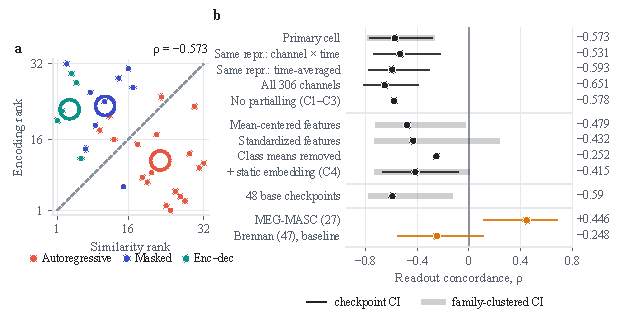
\includegraphics[width=\textwidth]{../figures_v2/integrated_20261010/fig03_concordance.pdf}
\caption{\textbf{The reversal is mostly between classes and survives representation and cell changes; its sign is unresolved after full feature standardization or C4.} (a)~Similarity rank against encoding rank
for the $32$ LibriBrain checkpoints (rank $1$ strongest); large rings mark each class's mean rank,
and the dashed diagonal is equal ranking. (b)~Readout concordance under each variant, LibriBrain in
black and the other two cohorts in amber. Thin bars: Fisher-$z$ intervals over checkpoints; thick
bars: family-clustered bootstrap intervals ($12$ families) where computed at submission (those of
MEG-MASC and Brennan, computed later, are in Table~\ref{tab:main}); a point without a bar
has no stored interval; hairlines separate groups of variants. Sources: \texttt{concordance32\_CORRECTED} and its variants;
\texttt{concordance32\_lb\_allch\_CORRECTED} (both readouts on all channels; the ledger's mixed-cell
entry is not plotted); \texttt{correction\_2026\_08\_derived} (no partialling);
\texttt{concordance32\_c4} (C4); and, re-extracted after a tokenization defect
(Appendix~\ref{app:extract-provenance}), \texttt{adr0006\_registered\_verdicts\_spacefix} and the
MEG-MASC receipt. Brennan is the registered per-epoch-baseline value (\texttt{brennan\_k2\_summary\_20261009}; Appendix~\ref{app:brennan-preproc}).}
\label{fig:concordance32}
\end{figure}

On LibriBrain the two readouts rank the $32$ checkpoints in
\emph{opposite} orders ($\rho=-0.573$). Both rankings are individually reliable ($0.98$ and $0.96$ against an attenuation
ceiling of $0.97$), so this is a disagreement between determined rankings. The family-clustered
$95\%$ CI, over $12$ units rather than $32$, is wider ($[-0.79, -0.26]$) and still excludes zero; with the added checkpoints re-extracted, the reversal also survives
the $48$-checkpoint base set that spans $2019$--$2026$ (Table~\ref{tab:main}), so the registered
falsifier that it was an artifact of older models did not fire.

The disagreement is about architecture \emph{classes} more than individual models
(Figure~\ref{fig:concordance32}a). Removing each class's mean from both readouts leaves a weak
within-class concordance, so, under the class-specific reading rule, $56\%$ of the effect is a between-class offset: similarity puts
autoregressive models last and encoding puts them first, a gap of $+25.7$ ranks that survives
permuting the architecture label over whole families. Autoregressive checkpoints are also wider,
but with width matched the gap shrinks and still survives the family-clustered test
(Appendix~\ref{app:mechanism}). Objective class also fixes how a checkpoint is read: masked and
encoder--decoder checkpoints read the whole sentence, including the words after the target. Read up to
the target word at its last token, as the causal ones are, the $14$ give $\rho=-0.016$ (family-clustered
CI $[-0.40, +0.34]$; registered, Table~\ref{tab:main}): the reversal holds for the readouts as
conventionally applied, and under a common reading rule it is not determined (Appendix~\ref{app:readrule}). On LibriBrain class also fixes
the tokenization rule, which changes $15$ of the $18$ autoregressive feature sets little
(Appendix~\ref{app:extract-provenance}). Neither representation nor cell explains it, and dropping the lexical
partialling does not either: handing both readouts the identical neural representation, scoring all
$306$ channels or dropping C1--C3 leaves the concordance close to its headline value
(Figure~\ref{fig:concordance32}b). With the static-embedding control C4 added it is $-0.415$, with a family-clustered
interval that includes zero: neither the reversal nor its change is determined (Table~\ref{tab:main}; Appendix~\ref{app:c4}).

\textbf{Feature geometry is not excluded.} Proposition~\ref{prop:invariance} predicts where to
look: cosine similarity weighs the dominant direction of anisotropic autoregressive models by its
variance, while standardized ridge does not see per-coordinate scale. Standardizing features before
similarity keeps the point estimate negative, but under the headline's own inference the
mean-centered interval barely excludes zero and the fully standardized one crosses it
(Figure~\ref{fig:concordance32}b). We therefore do not claim the reversal is independent of feature
geometry; the claim is that the readouts \emph{as conventionally applied} disagree. A post hoc
refit of ten models confirms parts (i)--(ii) on real data (centering changes similarity ranks and
leaves encoding scores unchanged to numerical precision) and shows that a sample-varying rank-one
addition does move encoding ranks. The old claim that
standardization absorbs that perturbation was false, and the synthetic perturbation
does not identify the endogenous cause (Appendix~\ref{app:mechanism}). Effective dimensionality covaries with
the readout gap within the autoregressive class only, which is exploratory. A third readout,
contrastive decoding, gives no determined ranking (Appendix~\ref{app:decoding}).

\textbf{The reversal belongs to one cohort.} This rests on MEG-MASC alone. With the same band,
window, depth and controls (right temporal sensors), its $27$ listeners give two determined readouts
and a \emph{positive} concordance whose family-clustered interval, the inference the headline is held
to, excludes zero, narrowly ($[+0.03, +0.71]$). Brennan EEG ($47$ listeners, all $60$ channels) adds no
second case. Its epochs, unlike LibriBrain's and MEG-MASC's, are neither filtered nor baseline-corrected
(raw FieldTrip slices), and on them the neural dissimilarities track the distance in story time between
words (median Spearman $+0.885$). With a per-epoch baseline the Brennan concordance is $-0.248$
(family-clustered CI $[-0.62, +0.14]$; linear detrend $-0.047$, $[-0.53, +0.39]$), not determined, and its
class gap ($+15.6$ ranks, family-clustered $p=0.012$) has LibriBrain's sign
(Appendix~\ref{app:brennan-preproc}); its signal-to-word alignment is verified on one listener
(Appendix~\ref{app:brennan}). Recording depth
does not explain the difference ($11$ of $12$ LibriBrain sessions reverse on their own,
Appendix~\ref{app:depth}), neural measurement quality does not either, and two further
pre-registered accounts were refuted (Appendix~\ref{app:refuted}). This is an
existence proof, not a field-wide constant.

\subsection{Additional Findings}\label{sec:appendix-findings}

\textbf{Scaling, retested at modern scale} (registered before extraction). Across three Qwen
generations \citep{qwen2024qwen25, yang2025qwen3, qwen2026qwen35}, $2.5$ ($0.5$B--$72$B), $3$ and $3.5$, in no generation does size order
both readouts positively on the primary cell (Appendix Figure~\ref{fig:scaling}). On the
largest ladder the ordering is itself readout-dependent: encoding falls with size ($72$B vs
$0.5$B, paired $p=0.0005$) while similarity rises ($p=0.001$). A post hoc, training-fold-expanded
ridge grid attenuates the encoding size correlation from $-0.964$ to $-0.464$, so that slope is
regularization-sensitive, while $72$B stays below $0.5$B (Appendix Table~\ref{tab:alpha-grid}). Scaling each
session's encoding target separately (Section~\ref{sec:fragility}) also flattens it: on cached features
$\rho=-0.79$, with $0.5$B--$32$B nearly level and the drop carried by $72$B (Appendix~\ref{sec:scorecard}). On
MEG-MASC's $27$ listeners the same rungs do not order similarity by size, and the encoding arm fails
its rankability gate, so it is not determined. The six-point Pythia ladder ($70$M--$2.8$B), scored
at the fixed depth, does not order encoding by size either (Appendix~\ref{sec:scorecard}). Over the
whole range, size-scaling claims made under
one readout \citep{antonello2024scaling, hong2026larger} do not describe both; across six
base--instruct twins instruction tuning shifts neither readout consistently ($2/6$, $4/6$;
exploratory). \textbf{A band comparison} (Appendix~\ref{sec:broadband}): broadband reaches a higher peak
alignment than $30$--$80$~Hz gamma in $206$ of $213$ recordings; on LibriBrain, where the ceiling
was measured, gamma has no reproducible word-level structure to align to. The $70$--$150$~Hz
intracranial envelope is not tested.
\textbf{Ten cross-setting hypothesis tests} (Appendix~\ref{sec:scorecard}) are conceptual extensions
and analogies, not a replication-rate estimate; one row lacks its source tensors and is unverified.

\subsection{Fragility of Score Computation}\label{sec:fragility}

A separate class of instability concerns how scores are computed: errors of this class produce
plausible numbers rather than exceptions. Four
occurred in this pipeline (Appendix~\ref{app:fragility}) with one cause, code written as if inputs were on a unit scale and
applied to neural data in physical units. The fourth was found after submission: the LibriBrain
encoding target was scaled once across sessions, two of which differ in scale ($76.6\times$ and
$5.5\times$ the median), which lowered every encoding score ($1.7$--$3.1\times$) and pinned the ridge penalty at its
grid ceiling; with each session scaled separately the concordance is $\rho=-0.543$ (family-clustered
CI $[-0.71, -0.22]$), so the reversal does not depend on it. The least visible of the first three, a $10^{-12}$ guard in a correlation
denominator, shrank stronger-predicting models less and changed the readout concordance of an
earlier analysis in this project from $-0.573$ to $-0.678$; changing only that constant recovers
$-0.573$. Our claim-reproduction harness read $97/97$ green throughout, because it checks stored
results against the paper's claims and cannot see that they came from defective code.
Reproducibility and correctness are different properties, and the first is routinely offered as
evidence of the second \citep{eklund2016cluster, botviniknezer2020variability}.


\section{Discussion and Limitations}\label{discussion}\label{limitations}

Across listeners rankings were stable; across readouts they reversed, as conventionally applied,
on the single LibriBrain listener (feature geometry not excluded; not determined under a common
reading rule) but not on MEG-MASC, and on Brennan EEG, once slow drift is removed, not determined;
across stories they held in one crossed cohort and, exploratorily, failed in the other. A claim that
a model is more brain-like should rest on both readouts, with standardized features as a geometry
check, on determined rankings with family-clustered intervals, and on a named cohort and stimulus sample, with
uncertainty over stimuli where the design allows; otherwise it is a claim about one readout, cohort
and text. None of this certifies a
mechanism \citep{murphy2026country}: the band result is a reliability-grounded preprocessing
correction, every scorecard verdict is our operationalization, and the stimulus result shows
rankings can fail to generalize across stimulus samples, not that the narrative causes it.

\emph{Single-subject where it is load-bearing.} LibriBrain, the primary cohort, is one listener
over many sessions, and it is where the broadband ceiling is computed. MEG-MASC reproduces the
ceiling ordering, but its word-level dissimilarity sits near the noise floor, leaving the
normalization's alignment side ill-defined: clean on one cohort, echoed on a second, not on all
five. \emph{Magnitude scale and in-sample selection.} Raw best-cell alignment is $10^{-3}$--$10^{-2}$ in MEG
and $\approx2\times10^{-2}$ in ECoG, and headline values select cells in-sample at a $6$--$85\%$ cost
(Section~\ref{sec:leaderboard}) with no held-out rebuild. \emph{Scope of the readout comparison.}
With C4 added, the fixed-depth reversal is not determined (CI including zero), and neither is it
under a common reading rule, every checkpoint read up to the target word ($\rho=-0.016$; Appendix~\ref{app:readrule}),
so it describes the class-specific reading rules. Of the two other cohorts only MEG-MASC is positive
under family-clustered inference, narrowly, so the cross-cohort contrast rests on it alone; Brennan's
epochs had no baseline, with one its sign is not determined (Appendix~\ref{app:brennan-preproc}), and its
alignment is verified on one listener (Appendix~\ref{app:brennan}). The
cross-cohort contrast also crosses the tokenization rule of autoregressive features and the encoding
fold (Appendices~\ref{app:extract-provenance},~\ref{app:depth}); unspaced-input
checkpoints were re-extracted except in ds003020 and other MEG-MASC and Brennan analyses.

\subsection*{AI Use Statement}

We used generative AI tools (Anthropic Claude and OpenAI Codex agents) to implement experiment
code and check it for correctness, to collect public datasets, to check references, and to polish
the writing. The authors take full responsibility for all content.

\subsection*{Ethics Statement}\label{ethics}

BrainLLM-Bench is built entirely on previously published human-recording datasets,
each collected under its own institutional ethics approval and participant consent:
LibriBrain, MEG-MASC, MEG-SCANS, the Brennan EEG corpus, and the ``Podcast''
intracranial dataset (OpenNeuro \texttt{ds005574}), whose original data papers we
cite; the crossed-narrative analysis also uses the public fMRI dataset ds003020
\citep{lebel2023natural}. We did not collect new human data. We will redistribute only
derived artifacts (per-word word lists, sensor-region maps and alignment tensors), never raw
recordings, and the word lists come from public narrative stimuli (audiobooks,
read stories and podcasts) that carry no participant-identifying content. The intracranial
cohort is the most sensitive; we use it only through the maintainers' de-identified
OpenNeuro release and report electrode locations only at the MNI-region level.
Brain--LLM alignment benchmarks carry a modest dual-use consideration, that better
alignment metrics could inform neural decoding of language; the effects here are
small and word-level, well short of message reconstruction, and we flag the concern
rather than dismiss it.

\subsection*{Reproducibility Statement}\label{reproducibility}

The quantitative headline results trace to files under the project's
\texttt{results/} directory; the unavailable baseline-comparison tensors in the historical
scorecard are an explicit exception. We verify stored summaries rather than rerun all analyses: the per-cohort headline cells and the broadband count to
\texttt{cross\_cohort\_summary.tsv} and \texttt{per\_unit\_bb\_vs\_gamma.tsv} (four
cohorts are scored under the full confound-controlled tensor protocol, and
Appendix Figure~\ref{fig:cohorts} reports exactly those four; Brennan EEG has no headline cell
under the tensor protocol, so it is absent from that figure, and it is scored on the fixed-depth
route, Table~\ref{tab:main} and \S\ref{sec:concordance}),
the per-band reliability ceiling to \texttt{p2\_perband\_ceiling.json}, the
cross-setting outcomes to \texttt{scorecard/\allowbreak scorecard\_\allowbreak transport.tsv} (legacy labels in
\texttt{scorecard/scorecard.tsv}), the family-clustered intervals of
\S\ref{sec:concordance} to \texttt{p4\_\allowbreak encoding/\allowbreak family\_\allowbreak clustered\_\allowbreak ci\_\allowbreak CORRECTED.txt} and, for the $48$ base checkpoints,
\texttt{p4\_\allowbreak encoding/\allowbreak space\_\allowbreak fix\_\allowbreak 20260925/\allowbreak aggregate/\allowbreak adr0006\_\allowbreak registered\_\allowbreak verdicts\_\allowbreak spacefix.json} (the
unspaced run: \texttt{concordance\_modern\_final\_v2.json}), and the family map to
\texttt{codes/model\_families.py}, the single definition every clustered inference imports. The protocol is deterministic
given a fixed random seed for the permutation nulls. The tensor harness takes public recordings
plus word lists and sensor-region maps. Its validation recomputes all $504$ stored per-(model,
session) values behind the LibriBrain cell to within $10^{-9}$ from cached neural dissimilarity
matrices, so it checks the model side, the confound partialling and the statistic but not the
neural preprocessing, and it has a portable known-answer test. This validates the tensor route, not
the C1--C3 fixed-depth sweep. That sweep's scores are reproducible from the cached features, and $31$ of its $32$ checkpoints
also by re-extraction: the $17$ autoregressive ones with the earlier extractor revision shipped in
the supplementary material, the $14$ others with the documented one (Appendix~\ref{app:c4}); GPT-2
small is matched by file identity. Re-extracting the autoregressive ones with the documented
revision does not reproduce them, because it tokenizes differently
(Appendix~\ref{app:extract-provenance}). Of the $25$ extension
checkpoints, $18$ were extracted with the documented extractor under a library version at which,
for their tokenizers, it removes the spaces between words (Appendix~\ref{app:extract-provenance});
all $25$ were re-extracted, with the receipts and gates in
\texttt{p4\_encoding/space\_fix\_20260925.json}. The checks added in this revision read
\texttt{readrule\_20260926/} (reading rule), \texttt{alpha32\_20260926/} (ridge range) and
\texttt{paperA\_rebuttal\_20261004/} (per-session target scale, Qwen2.5 ladder, Brennan alignment and
preprocessing, seed sweeps). A subset is released at \coderepo: the harness and its stored-result checks ($198$ registered claims; the run marks the $33$ that pin superseded values kept for provenance,
$25$ of them values computed on the unspaced features, and the $53$ that belong to a separate
boundary-effect analysis not part of this submission), the checker for Table~\ref{tab:main}, the
derived result files and scorecard cited above, the seventeen pre-registration documents (ADR 0001--0010, one of them an amendment; the readout-concordance test; the C4 control; the re-extraction; the reading rule; the ridge range; the post-submission checks; the rescaled Qwen2.5 ladder), the sensor-region
atlases and the analysis scripts. The alignment tensors, word lists, cached model features and
cached neural dissimilarity matrices are not in it, so the $504$-value validation cannot be rerun from
it; they will be released later with an archival DOI.

\bibliographystyle{iclr2027_conference}
\bibliography{references}

\appendix
\section{Proof of Proposition~\ref{prop:invariance}}\label{app:proof}

Throughout, the neural patterns, the brain dissimilarity $D^{\mathrm b}$ and the confound
matrices $C_1$--$C_3$ do not depend on the model features, so a readout score is unchanged whenever
the model-side object it is computed from is unchanged.

\textbf{(i)} For $c>0$ and orthogonal $Q$, $\langle cQ^\top x_i, cQ^\top x_j\rangle=c^2\langle
x_i,x_j\rangle$ and $\|cQ^\top x_i\|=c\|x_i\|$, so every cosine, hence $D^{(m)}$ and the partial
Spearman correlation of Eq.~\eqref{eq:rsa}, is unchanged. For the converse it suffices to exhibit
one case. For $x_1=(1,0)$, $x_2=(0,1)$, $x_3=(2,1)$ the cosine distances are
$d_{12}=1$, $d_{13}=1-2/\sqrt5\approx0.106$, $d_{23}=1-1/\sqrt5\approx0.553$, so
$d_{13}<d_{23}<d_{12}$. Translating by $b=(0,2)$ gives $d_{12}\approx0.106$, $d_{13}\approx0.008$,
$d_{23}\approx0.168$, so $d_{13}<d_{12}<d_{23}$; rescaling by $\operatorname{diag}(1,3)$ gives
$d_{23}\approx0.168<d_{13}\approx0.445<d_{12}=1$. Both maps change the rank order of the word-pair
dissimilarities, so, embedded in a larger word set with a suitable $D^{\mathrm b}$ and confounds, they
change the partial Spearman statistic.

\textbf{(ii)} Let $X'=XA+\mathbf 1b^\top$ with $A=\operatorname{diag}(a)$, $a_j>0$. On the training
fold the column means and deviations become $\mu'=A\mu+b$ and $\sigma'=A\sigma$, so
$\tilde X'=(XA+\mathbf 1b^\top-\mathbf 1\mu^\top A-\mathbf 1b^\top)A^{-1}\Sigma^{-1}=\tilde X$ on both
training and held-out rows. The standardized design is identical, so the selected $\alpha$,
$\hat W_\alpha$ and the held-out predictions are identical at every $\alpha$. (The implementation
adds $10^{-8}$ to $\sigma$; the identity then holds up to that guard.) Now let $A$ be any
invertible matrix and write $Z=\tilde X_{-u}$, $Z_u=\tilde X_u$. Centering commutes with right
multiplication, and per-column scaling is right multiplication by a positive diagonal matrix, so
$Z'=ZB$ and $Z'_u=Z_uB$ with $B=\Sigma A\Sigma'^{-1}$ invertible. If $Z$ has full column rank, the
$\alpha\to0$ limit of Eq.~\eqref{eq:ridge} is the least-squares solution and
\[
Z'_u(Z'^\top Z')^{-1}Z'^\top\tilde Y_{-u}=Z_uB\,B^{-1}(Z^\top Z)^{-1}B^{-\top}B^\top Z^\top\tilde Y_{-u}
=Z_u(Z^\top Z)^{-1}Z^\top\tilde Y_{-u},
\]
so the held-out predictions, and the Pearson score computed from them, are unchanged.

\textbf{(iii)} With $Z=\sum_k s_k u_kv_k^\top$, $Z^\top Z+\alpha I=\sum_k(s_k^2+\alpha)v_kv_k^\top
+\alpha P_\perp$, where $P_\perp$ projects onto the orthogonal complement of the right singular
vectors; since $Z^\top\tilde Y_{-u}$ lies in their span, the training-fold fitted values are
$Z\hat W_\alpha=\sum_k s_k u_kv_k^\top\sum_l(s_l^2+\alpha)^{-1}s_l v_lu_l^\top\tilde Y_{-u}
=\sum_k\frac{s_k^2}{s_k^2+\alpha}u_ku_k^\top\tilde Y_{-u}$.

\textbf{(iv)} Let $\bar X$ be the centered features, $n$ words. The nonzero eigenvalues of the Gram
matrix $K=\bar X\bar X^\top$ are those of $\bar X^\top\bar X=n\,\mathrm{Cov}$, namely $n\lambda_k$,
and $K=\sum_k n\lambda_k v_kv_k^\top$ with orthonormal $v_k$, so the rank-one terms are orthogonal in
the Frobenius inner product and $\|K\|_F^2=n^2\sum_k\lambda_k^2$. The leading term's share is
$\lambda_1^2/\sum_k\lambda_k^2$. Because $0\le\lambda_k\le\lambda_1$, $\sum_k\lambda_k^2\le
\lambda_1\sum_k\lambda_k$, which gives both $\lambda_1^2/\sum_k\lambda_k^2\ge\lambda_1/\sum_k\lambda_k$
and $1/\mathrm{PR}=\sum_k\lambda_k^2/(\sum_k\lambda_k)^2\le\lambda_1/\sum_k\lambda_k$. Chaining the two,
the share is at least $1/\mathrm{PR}$. \hfill$\square$

\textbf{Scope.} Parts (i)--(iii) are exact statements about the pipeline of
Section~\ref{sec:setup}, except that (ii)'s second claim is an $\alpha\to0$ limit, whereas the
scored $\alpha$ is selected from a grid. Part (iv) concerns the centered inner-product geometry;
cosine distance is taken on uncentered features and divides by each word's norm, so (iv) motivates, and does not prove, the
reading that a low-participation-ratio model's similarity score is dominated by one direction. None
of the four parts says which transformation separates the models in our data; that question is
the empirical one of Appendix~\ref{app:mechanism}, and it remains open.

\section{Benchmark Context and Protocol Matrix}
\subsection{Prior Work and Benchmark Comparison}\label{app:related-benchmarks}

\textbf{Brain--LLM alignment studies.} A large body of work relates
language-model features to brain responses through encoding models
\citep{schrimpf2021neural, caucheteux2023evidence, antonello2024scaling, toneva2019interpreting,
goldstein2022shared}, representational similarity \citep{kriegeskorte2008representational,
nili2014toolbox}, and decoding \citep{tang2023semantic, defossez2023decoding}. In vision,
conclusions flip with the similarity measure \citep{soni2024conclusions, ahlert2024aligned}. These efforts differ in cohort, modality, model, statistic and
preprocessing, so their magnitudes sit on incompatible scales \citep{oota2024survey}.

\textbf{Existing benchmarks.} The integrative-modeling line \citep{schrimpf2021neural}
scores many models against fixed brain recordings and is the closest prior benchmark in
spirit. It ranks models with one primary metric (encoding predictivity), single-modality within
each dataset, and carries no built-in confound battery or per-band reliability ceiling. It does
check that metric: its scores generalize to a dissimilarity-matrix metric that involves no fitting,
for untrained models too, and model scores correlate across datasets ($r = 0.94$ between the two
Pereira2018 experiments, $r = 0.50$ between Pereira2018 and Fedorenko2016).
% VERIFY-SCHRIMPF: the RDM-generalization statements and r = 0.94 / 0.50 were read in the main text
% (PMC8694052, 2026-10-07), which cites SI Appendix Figs. S2A and S8D for them; the SI itself returned
% HTTP 403 and was not opened, so the SI locators are left out and how "generalize" is quantified
% (e.g. whether it is a rank correlation over models) is unverified. Author: check on the PNAS PDF + SI.
What it does not report is a rank concordance between readouts on matched checkpoints with a
rankability precondition; brain-tuning and
driving-response studies \citep{moussa2025braintuning, tuckute2024driving} likewise use one
readout. Whether two readouts, each with a determined ranking, order the same language models alike
(in vision, \citet{soni2024conclusions} and
\citet{ahlert2024aligned} show that they need not) is the question our readout comparison asks; the ML-side leaderboard-reliability
literature that motivates treating participants and stimuli as two sampled axes is reviewed in
Appendix~\ref{app:related-ml}. BrainLLM-Bench differs on four axes: it scores similarity and encoding side by side on its
primary cohort (and reports why decoding does not yet yield a determined ranking), so their
concordance is measured rather than assumed; it spans modalities (MEG, EEG, ECoG)
and languages within one protocol; it carries confound control and reliability ceilings
inside the score rather than as add-ons; and it treats the frequency band as a benchmarked
dimension rather than a fixed preprocessing choice.

\textbf{The reliability critique.} The confound and reproducibility critiques
\citep{feghhi2026spurious, lai2025illusions} directly motivate a standardized frame. We take their
lesson, that positional, word-rate and other simple stimulus features must be controlled before an
alignment score is read, and build confound control and clustered inference into the measurement
rather than adding them post hoc: every tensor cell is scored with the confound battery available
and every null is clustered; raw best-cell values are reported separately and labelled as such.


\subsection{Executed Route Matrix}
Table~\ref{tab:protocols} lists the executed analysis routes, what each controls, and which one the
portable validation covers.
\begin{table}[t]
\centering\small
\begin{tabular}{@{}p{2.6cm}p{3.7cm}p{5.0cm}@{}}
\toprule
Analysis & Scoring and layer rule & Controls and validation scope \\
\midrule
Original tensor & Partial RSA across layer/cell grid; raw argmax shown descriptively & C1--C4; per-band ceilings and $27$-cell inference grid. The portable tensor validation checks this route. \\
Fixed-depth sweep & RSA and held-out ridge encoding; relative depth $0.5$ & RSA: C1--C3 (C1--C4 for the $32$, Appendix~\ref{app:c4}); encoding: train-fold standardization. $32$ then $57$ checkpoints; model-family clustered comparisons. \\
Crossed stimuli & Same fixed-depth scores, separately by stimulus (ds003020: word features averaged per TR) & C1--C3 RSA (ds003020: C1--C2); encoding leaves a listener out (ds003020: shuffled five-fold TR splits within a story and listener); listener and stimulus resampling reported separately. MEG transfer result exploratory. \\
\bottomrule
\end{tabular}
\caption{Executed analysis routes. C1--C3 are length, frequency and orthography; C4 is model-specific
static embedding. With C4 added, the $32$-checkpoint fixed-depth reversal is not determined
(Appendix~\ref{app:c4}); the $57$-checkpoint sweep and the MEG-MASC crossed-stimulus scores use C1--C3; ds003020 uses C1--C2.}
\label{tab:protocols}
\end{table}
\section{Model-Size Ladder Visualization}
Figure~\ref{fig:scaling} shows the three Qwen ladders of Section~\ref{sec:appendix-findings}, one row
per readout.
\begin{figure}[t]
\centering
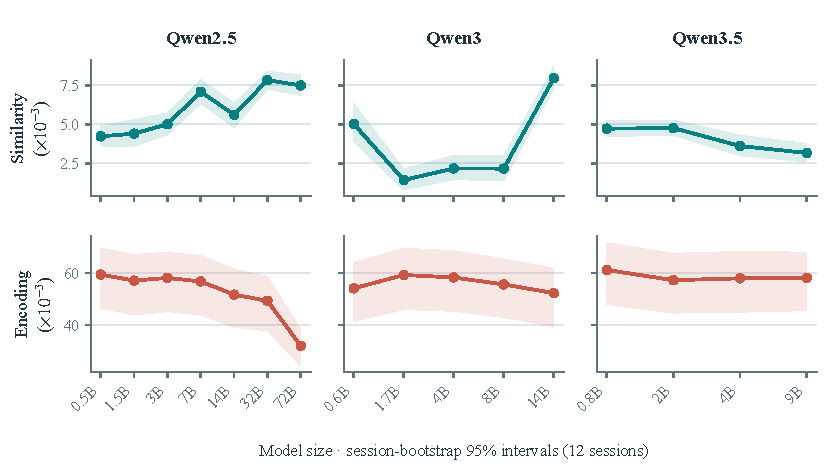
\includegraphics[width=1.0000\textwidth]{../figures_v2/integrated_20260926/fig_scaling_spacefix.pdf}
\caption{\textbf{Three model-size ladders, separated by readout.} Similarity (top) and encoding (bottom) use shared scales within each row; the two rows have different ranges. Points are per-session means, ribbons are session-clustered bootstrap 95\% intervals (12 sessions). Each generation retains its published rungs. Values are read from concordance\_spacefix\_libribrain.json (every extension rung re-extracted after the tokenization defect, Appendix~\ref{app:extract-provenance}); the registered tests, rather than visual slope alone, determine the claims. These curves use the original bounded 1e1--1e6 ridge grid; expanded-grid sensitivity is reported separately in the text.}
\label{fig:scaling}
\end{figure}


\section*{Summary of Findings}

The appendices below report in full the findings summarized in the main text.
Figure~\ref{fig:concordance} collects the six-family readout diagnostic behind
Appendix~\ref{app:decoding} and the corrected Pythia ladder of Appendix~\ref{sec:scorecard}.

\begin{figure}[t]
\centering
\includegraphics[width=1.0000\textwidth]{../figures_v2/integrated_20260923/fig04_redrawn.pdf}
\caption{\textbf{Readout-dependent ranks and a receipt-backed size ladder.} (a) The six-family legacy diagnostic, with decoding ranked by the mean of twelve leave-one-session-out retrains. The decoding order is not stable (split-half reliability 0.54); RSA and encoding reliability are both 0.94. This legacy diagnostic predates the correction of Appendix~\ref{app:fragility} and was not recomputed with it. (b) The corrected six-rung Pythia encoding ladder at preregistered depth, with session-bootstrap 95\% intervals. This replaces the old illustrative three-point peak-normalized panel, whose RSA values were hand-entered. Source: concordance.json, decoding\_lb\_persess.json, scaling\_ladder\_test\_CORRECTED.json.}
\label{fig:concordance}
\end{figure}

\section{Protocol Parameters}\label{app:protocol}

Sessions are subsampled to at most $2500$ words under a fixed seed before the dissimilarity
matrix is built, which bounds the dissimilarity vector at $12.5$~MB and is what keeps the tensor
tractable. The per-band reliability ceiling is computed on a separate, smaller repeated-word cache
($462$ words over $12$ sessions), since a split-half ceiling needs words that recur across
sessions. Word epochs run from $-200$ to $+800$~ms around onset. For the per-band reliability
analyses (the ceiling and Appendix~\ref{sec:broadband}) each epoch is filtered into six bands with a
fourth-order Butterworth filter: broadband $1$--$80$, delta $1$--$4$, theta $4$--$8$, alpha $8$--$13$,
beta $13$--$30$, and gamma $30$--$80$~Hz. The alignment tensor and the fixed-depth readout comparison
filter the narrow bands the same way but apply no filter for broadband, which there is the stored
epoch: baseline-corrected for LibriBrain and MEG-MASC, and neither filtered nor baseline-corrected for
the Brennan rebuild (Appendix~\ref{app:brennan-preproc}). Sensors are partitioned into six
anatomical wedges (frontal, temporal, parieto-occipital $\times$ left, right) by fixed sensor-layout
atlases for the Neuromag-306 and KIT-208 systems (in the bundle); scalp EEG uses all channels; ECoG uses language
regions of interest (ROIs) in MNI (Montreal Neurological Institute) standard space.

\paragraph{Test family and multiplicity.} Each confirmatory question in the main text --- the
concordance-versus-ceiling test, the crossed-narrative dispersion test, the scaling ladders, and
the modern-set reversal --- has one registered primary statistic with a decision rule fixed
before scoring, so its confirmatory test family has size one and we apply no family-wise
correction across questions; no error-rate guarantee is therefore claimed across questions, and an
exploratory analysis does not rescue a registered test that failed. Within a question, the only test family larger than one is the
$27$-cell LME grid, controlled at Benjamini--Hochberg FDR \citep{benjamini1995controlling} $q = 0.05$ over the $27$ cells within
each cohort~$\times$~model. Every other $p$-value in the paper is descriptive, and an analysis
labelled \emph{exploratory} (the story-transfer finding whose registered primary did not
confirm, the participation-ratio mechanism, and the base--instruct twins) carries no
confirmatory weight, whatever its $p$-value. The family map is a single module imported by every
clustered inference (\texttt{codes/model\_families.py}); it folds DistilBERT and ALBERT into
BERT, since they share its corpus and tokenizer lineage, giving $12$ families rather than the
$14$ a name-level split would give --- fewer resampling units and wider clustered intervals,
which is the conservative side when the claims rest on those intervals excluding zero. The
registration documents are internal and shipped in the supplementary material. Only the $32$-checkpoint registration predates the
reversal (it was written when a six-family pilot existed); the later ones, including the
$48$-checkpoint, C4 and re-extraction registrations, were written after it was known, so those that
concern the reversal test the robustness of a known effect in the same listener and do not
replicate it. Table~\ref{tab:checkpoints} lists the $32$ checkpoints by class and family.

\begin{table}[t]
\centering\small
\caption{The $32$ checkpoints of the readout comparison, by objective class and family; the
$12$ families are the resampling units of every family-clustered interval. All are the public pretrained releases.}
\label{tab:checkpoints}
\begin{tabular}{@{}llp{6.4cm}@{}}
\toprule
Class & Family & Checkpoints \\
\midrule
Autoregressive ($18$) & GPT-2 \citep{radford2019language} & small, medium, large, XL \\
 & Pythia \citep{biderman2023pythia} & 70M, 160M, 410M, 1B, 1.4B, 2.8B \\
 & OPT \citep{zhang2022opt} & 125M, 350M, 1.3B \\
 & GPT-Neo \citep{black2021gptneo} & 125M, 1.3B \\
 & Llama \citep{grattafiori2024llama3} & Llama-3.2-1B \citep{meta2024llama32} \\
 & Qwen \citep{qwen2024qwen25} & Qwen2.5-0.5B, Qwen2.5-1.5B \\
\midrule
Masked ($9$) & BERT \citep{devlin2019bert} & base, large; DistilBERT \citep{sanh2019distilbert}; ALBERT-base-v2 \citep{lan2020albert} \\
 & RoBERTa \citep{liu2019roberta} & base, large \\
 & DeBERTa \citep{he2023debertav3} & v3-base, v3-large \\
 & ELECTRA \citep{clark2020electra} & base discriminator \\
\midrule
Encoder--decoder ($5$) & T5 \citep{raffel2020t5} & small, base, large \\
 & BART \citep{lewis2020bart} & base, large \\
\bottomrule
\end{tabular}
\end{table}

\paragraph{Compute.} Everything downstream of feature extraction runs on one CPU workstation; no
analysis stage needs a GPU. Language-model feature extraction for the $32$-checkpoint sweep is the
only GPU stage, embarrassingly parallel over (model, narrative) pairs; features are extracted once
and cached, and every result in this paper is computed from those caches.

\paragraph{Feature-extraction provenance.}\label{app:extract-provenance} Every checkpoint is read
at the same relative depth, but the reading procedure depends on the class
(\texttt{extract\_llm\_layers\_multi.py}): causal models read the prefix that ends in the target
word and are read at its last token; masked models read the whole sentence, including the words
after the target, and the target's sub-tokens are averaged; encoder--decoder models are read the
same way through the encoder stack alone. Objective class therefore also fixes context direction and
token pooling, so the between-class component of the reversal (Section~\ref{sec:concordance}) cannot
be attributed to the training objective alone (tested below, under a common reading rule). Among causal models, what differs is how the prefix
is tokenized. Two rules were used. The \emph{joined-string} rule passes the prefix as one string with the tokenizer's default
settings; it wrote the LibriBrain features of the $18$ autoregressive checkpoints of the
$32$-checkpoint sweep ($17$ by an earlier revision of the documented extractor
\texttt{extract\_llm\_layers\_multi.py}, shipped in the supplementary material, and GPT-2 small by
the older single-model \texttt{extract\_llm\_layers.py}). The \emph{word-list} rule of the
documented revision (\texttt{is\_split\_into\_words}, \texttt{add\_prefix\_space}) was introduced to
fix target-word alignment in the masked and encoder--decoder models; it wrote the LibriBrain
features of those $14$ checkpoints, of all $25$ checkpoints of the registered extensions ($16$ base,
$9$ post-trained), and of every checkpoint on MEG-MASC, Brennan and ds003020 (the $27$- and
$47$-listener analyses re-index those features rather than re-extracting them). This attribution
rests on the extraction code and job history, not on recomputed features. For the GPT-2 tokenizer,
and Pythia's under a nearby library version, the two rules differ only in whether the
sentence-initial word carries a leading space. For the Qwen and Llama tokenizers under transformers
$4.57.1$, the library version of most extraction runs, the word-list rule inserts no space between
words: in two LibriBrain test batches every non-initial word lost its leading space ($252/252$ word
boundaries for each of the $18$ Qwen and Llama tokenizers probed; the other checkpoints extracted
under that version share those tokenizer files), so the model reads, for example,
``Intheyeareighteen\ldots''; the read-out token is still the last sub-token of the target word, in
its space-less form. The Qwen3.5 checkpoints and one other post-trained checkpoint were extracted
under transformers $5.15.0$, where the same probe loses no space ($0/252$), so they read spaced
text. The $14$ masked and encoder--decoder tokenizers lose no space under this rule
($0$ of $46{,}511$ word boundaries each, in $2{,}000$ LibriBrain sentences). Rerunning the documented extractor on the $30{,}000$ scored LibriBrain
words leaves the $14$ masked and encoder--decoder rows unchanged (median row cosine $1.0000000$
for all $14$) and changes the autoregressive rows: per checkpoint, $36\%$ (GPT-Neo-125M) and
$93$--$99.8\%$ (the other $17$) of rows fall below cosine $0.9999$ with the cached rows, and the
median row cosine is $0.9965$--$0.9999$ for the $15$ GPT-2, Pythia, OPT and GPT-Neo checkpoints and
$0.786$ (Llama-3.2-1B), $0.855$ and $0.897$ (Qwen2.5-0.5B, -1.5B), whose cached rows come from
spaced text and whose re-extracted rows from unspaced text. Three consequences follow.
(i)~On LibriBrain the rule is collinear with objective class among the $32$ checkpoints, so the
between-class component of the reversal (Section~\ref{sec:concordance}) is not separated from it.
(ii)~The autoregressive checkpoints were tokenized under the joined-string rule on LibriBrain and
under the word-list rule elsewhere, and Llama-3.2-1B and Qwen2.5-0.5B/1.5B first read unspaced text on
MEG-MASC, Brennan and ds003020 (including the listener and story analyses of Table~\ref{tab:main})
but not on LibriBrain, so the cross-cohort contrast also crosses the two rules. (iii)~Of the $25$
extension checkpoints, $18$ were first scored on unspaced text: $12$ of the $16$ base checkpoints added in
the $48$-checkpoint test (Qwen2.5 $3$B--$72$B, Llama-3.1-8B and -70B, the five Qwen3 base
checkpoints) and $6$ of the $9$ post-trained ones, so both members of five of the six base--instruct
twins; the Qwen3.5 ladder and its twin were not. The Qwen3 ladder, all seven rungs of the Qwen2.5
ladder on MEG-MASC and the $3$B--$72$B rungs of the LibriBrain Qwen2.5 ladder were first scored on
unspaced text, while the LibriBrain $0.5$B and $1.5$B rungs were not, so on those features the
$72$B-versus-$0.5$B contrast compared the two input conditions.
\emph{Re-extraction.} Under a pre-registration written after the defect was found and before any
re-extracted feature existed (\texttt{PREREG\_space\_fix\_reextract\_20260925.md}), all $25$
extension checkpoints ($18$ to repair the defect, $7$ to put every autoregressive LibriBrain
checkpoint under one rule), the MEG-MASC Qwen2.5 ladder and the three small checkpoints on MEG-MASC
and Brennan ($36$ extractions) were re-extracted with the joined-string rule. All $36$ passed the
tokenization gate (every row decodes to the spaced text) and the scorer-identity gate (the scorer
reproduces every published per-session value on the cached features); the $25$ LibriBrain extension
extractions, whose weight load also produced the MEG-MASC ladder rows, passed a weight-identity gate
(the documented rule on the same loaded weights reproduces the cached rows), and for the three small
checkpoints the new code path reproduced their cached LibriBrain features bit for bit. Every registered outcome
below uses the re-extracted features. Each follows the pre-registered rule
(\texttt{p4\_encoding/space\_fix\_20260925.json}). On the unspaced features, for comparison: the
$48$-checkpoint test gave $\rho=-0.58$ (family-clustered CI $[-0.78,-0.14]$; re-extracted $-0.59$,
$[-0.78,-0.12]$); the LibriBrain Qwen2.5 ladder gave encoding $\rho=-0.89$ and similarity $+0.61$
($-0.96$ and $+0.93$); the Qwen3 ladder's registered label was ``mixed'' (now ``not supported''; re-extracted, the
per-generation test gives, with session-clustered $95\%$ CIs, Qwen2.5 similarity $\rho=+0.93$
$[+0.82,+0.96]$ and encoding $-0.96$ $[-1.00,-0.82]$, Qwen3 $+0.30$ $[+0.30,+0.40]$ and $-0.40$
$[-0.70,0.00]$, Qwen3.5 $-0.80$ $[-1.00,-0.80]$ and $-0.20$ $[-1.00,-0.20]$, and no generation is
``supported''; with this few rungs the session bootstrap of a rank correlation takes few values, so an interval endpoint can equal the point estimate);
the base--instruct twins gave $3/6$ and $4/6$ ($2/6$, $4/6$); the MEG-MASC and Brennan
concordances were $+0.489$ $[+0.17,+0.72]$ and $+0.342$ $[-0.01,+0.62]$ ($+0.446$ $[+0.12,+0.69]$
and $+0.366$ $[+0.02,+0.63]$; on Brennan epochs without a baseline the interval then excluded zero,
narrowly, and with one the Brennan concordance is not determined, Appendix~\ref{app:brennan-preproc}). A descriptive check
in the pre-registration expected the $7$ extension checkpoints that already read spaced text to
change by a median row cosine of at least $0.99$; $6$ of the $7$ changed by more (median row cosine $0.978$--$0.986$;
the unspaced ones $0.851$--$0.919$), more than the first-word difference alone produced for the
GPT-2-type checkpoints, so by the pre-registered rule their classification as spaced is not confirmed by this check and
rests on the tokenizer probe alone; all $7$ were re-extracted, so no reported number depends on it. ds003020 and the MEG-MASC story, listener-half and
crossed-narrative analyses were not re-run, nor were the repeat-removal analysis
(Appendix~\ref{app:refuted}), the Brennan segment reliabilities (Appendix~\ref{sec:partition}) and the
Brennan class gap (Appendix~\ref{app:mechanism}); all still include the three unspaced checkpoints; the
other $15$ autoregressive checkpoints on MEG-MASC, Brennan and ds003020 keep the word-list rule. C4
was not rerun. The $32$-checkpoint LibriBrain headline read spaced text throughout and is unchanged.
Re-extracting the $17$ autoregressive checkpoints with the shipped earlier revision reproduces
their cached rows (Appendix~\ref{app:c4}, Deviation~2); re-extracting them with the documented
revision would not reproduce the reported fixed-depth scores exactly.

\paragraph{Common reading rule (registered).}\label{app:readrule}
Objective class also fixes how a checkpoint is read: causal checkpoints read the prefix ending in the
target word at its last token; masked and encoder--decoder checkpoints read the whole sentence,
including the words after the target, and average the target's sub-tokens (encoder stack only for
encoder--decoder models). Re-reading the $14$ masked and encoder--decoder checkpoints under the causal
rule (prefix ending in the target word, last sub-token; table below) gives
$\rho = -0.016$, family-clustered CI $[-0.40, +0.34]$ including zero, so under a common reading rule
the reversal is not determined. The test was registered before any feature under the new rule existed
(\texttt{PREREG\_readrule\_20260926.md}); its result was computed and committed about two hours before
the submission deadline and was not integrated into the submitted version, which said that no test
separated the reading rule from class. Everything else is the headline's: the same $30{,}000$ words,
$12$ sessions, cell, depth and scorers, with the $18$ causal checkpoints taken unchanged and the
tokenization rule still differing by class. All $14$ re-extractions passed the registered
scorer-identity, extraction-identity, target-alignment and completeness gates on one device class
(CPU). Both rankings stay reliable (split-half $0.981$ for similarity, $0.941$ for encoding), so the
open interval is not a loss of ranking variance. Relative to $-0.573$ the paired change is $+0.557$
(family-clustered CI $[+0.20, +0.82]$). The two secondary rules, registered as descriptive, place the
change: reading the whole sentence at the target's last sub-token gives $-0.663$ (family-clustered CI
$[-0.82, -0.36]$), and reading the prefix with sub-token averaging gives $-0.032$ ($[-0.42, +0.33]$),
so, descriptively, the change follows the words after the target rather than sub-token pooling. Under
the common rule all $14$ checkpoints rise in encoding and $9$ fall in similarity, the within-class
concordance is $+0.03$, and the between-class share ($56\%$ under the published rule) is undefined
at $\rho\approx0$.

\begin{center}
\footnotesize\setlength{\tabcolsep}{4pt}
\begin{tabular}{@{}llrcc@{}}
\toprule
Masked and enc--dec input & target vector & $\rho$ & family-clustered CI & paired $\Delta$ vs $-0.573$ \\
\midrule
whole sentence (published) & sub-token mean & $-0.573$ & $[-0.79, -0.26]$ & --- \\
prefix to the target (primary) & last sub-token & $-0.016$ & $[-0.40, +0.34]$ & $+0.557$ $[+0.20, +0.82]$ \\
prefix to the target (descriptive) & sub-token mean & $-0.032$ & $[-0.42, +0.33]$ & $+0.541$ $[+0.19, +0.82]$ \\
whole sentence (descriptive) & last sub-token & $-0.663$ & $[-0.82, -0.36]$ & $-0.089$ $[-0.25, +0.00]$ \\
\bottomrule
\end{tabular}
\end{center}
\noindent{\footnotesize Readout concordance over the $32$ LibriBrain checkpoints when the $14$ masked and
encoder--decoder checkpoints are read under each rule; the $18$ causal checkpoints always read the
prefix at its last token. Family-clustered intervals resample the $12$ families ($10{,}000$ draws,
seed $0$); $\Delta$ uses the same draws for both concordances. Checkpoint-level Fisher-$z$ interval of
the primary: $[-0.36, +0.33]$. Receipts: \texttt{readrule\_20260926/readrule\_summary.json} and one
gate-and-score receipt per checkpoint. (Set without a table number so that the submitted version's
table numbers are kept.)}

The $27$-cell inference grid is three left-hemisphere regions (temporal, frontal,
parieto-occipital) $\times$ three bands (delta, theta, gamma) $\times$ three layer groups
(phonological, syntactic, semantic). It is a deliberate subset of the full tensor, fixed in
advance.



\section{Full Per-Cohort Leaderboard}\label{app:leaderboard}


Table~\ref{tab:percohort} is the per-cohort leaderboard, a descriptive summary
rather than the paper's headline finding (that is the readout-dependence of
\S\ref{sec:concordance}): the best-aligning cell for each cohort~$\times$~model,
with its region, band, layer, latency, and the count of mixed-effects survivors. Two facts stand out. First, absolute
alignment is small and modality-ordered: MEG best-$\rho$ ranges $0.002$ to
$0.013$, and intracranial ECoG is the largest at $0.015$ to $0.022$, the
expected invasive advantage (Appendix Figure~\ref{fig:cohorts}). Second, the winning band
is broadband in $11$ of the $12$ cohort~$\times$~model cells; the only cell that
peaks elsewhere is LibriBrain-BERT at delta, a neighboring low-frequency band.
The peak latency spans $275$ to $768$~ms post-onset, with $9$ of the $12$ cells
between $340$ and $590$~ms, and the peak region is lateral temporal in every MEG
cohort, so the benchmark reproduces the
lateral-temporal, mid-latency word-alignment cell that the field expects, now
under one protocol across the four cohorts carried through it. A per-model leaderboard on the LibriBrain
headline cell (Appendix Figure~\ref{fig:leaderboard}) orders the three architectures scored on
LibriBrain (best band per model) by raw alignment; BERT-base leads at $13.1\times10^{-3}$, above the
three-times-larger GPT-2-medium ($6.9\times10^{-3}$), a size-versus-architecture
anomaly that Appendix~\ref{sec:scorecard} returns to. This
ordering is on raw alignment and is descriptive: the confound-controlled partial
that gates significance is near-null at the group mean
(\S\ref{sec:broadband}), so the leaderboard ranks models by an uncontrolled
quantity and should be read as ``which model aligns most before confound control,''
not as a validated brain-likeness score. The distinction is not cosmetic: BERT tops
this raw leaderboard, but under the confound-controlled similarity readout of the
$32$-model protocol the highest-ranked models are encoder--decoder and masked ones
(T5-small at $11.1\times10^{-3}$, ahead of DeBERTa and BART), with the autoregressive
family last --- the class ordering of \S\ref{sec:concordance}, not this one. So the
leaderboard's winner is confound-control-dependent --- a separate axis from the
assay-dependence of \S\ref{sec:concordance}, pointing the same way: the ranking is a
property of the measurement choice as much as of the model.

A third dependence is larger than either, and we measure it rather than assert it. The best cell
in Table~\ref{tab:percohort} is chosen on the same data its value is read from, so the printed
$\rho$ is an optimistically selected quantity. We price that on the two cohorts whose tensors we
can rebuild, choosing the cell on every unit but one and reading it on the held-out unit.

The cost depends on the cohort, not the statistic. Across nine ECoG patients with different
electrode coverage, held-out alignment collapses from $9.6$ to $1.4\times10^{-3}$ --- about $85\%$
is selection, and BERT-base's held-out estimate is slightly negative, indistinguishable from no
alignment. Across thirty-six recordings of one MEG listener it costs almost nothing, $6.4$ to
$6.0\times10^{-3}$, about $6\%$. Which cell wins explains the gap: on LibriBrain, in the rebuilt
$864$-cell grid used for this held-out test, all three models pick left-temporal broadband, beside the pre-registered cell, and leave-one-out reselects it in
nearly every fold, whereas across patients the argmax moves with the electrodes. Restricting the
LibriBrain search to $k$ random cells shows this is not a search-space effect --- the penalty stays
near zero from $k=16$ to $k=864$. The cohorts differ in grid and word budget, so we compare the
in-sample-to-held-out ratio within each, not absolute values across them.

Unit \emph{count} is a competing explanation the search-space control does not address, since it
varies the cells searched rather than the units averaged. Varying count directly, by subsampling
MEG-SCANS by subject with everything else fixed, the tax rises steeply as units are removed:
$13.3\%$ at twenty-three subjects, $34.4\%$ at nine, $53.2\%$ at four (Spearman $\rho = -0.96$
against subject count, $p < 0.001$). Count therefore reproduces much of the $85\%$-versus-$6\%$
contrast. A residual survives --- at a matched nine units ECoG still pays $85\%$ against $34.4\%$ ---
so heterogeneity contributes too, but our cohorts vary both at once and cannot separate them. The
supported claim is the weaker one: best-cell values are optimistically selected estimates, most optimistic in small cohorts of
dissimilar units, which describes the small intracranial studies where this reporting style is most
common. It is why the primary metric is defined at a pre-registered cell rather than the argmax.

Two honest reads of Table~\ref{tab:percohort} belong with it. The survivor counts split by
direction, and for MEG-MASC GPT-2 all six FDR survivors are negative-direction, so its positive
best-cell is not backed by positive population evidence; two further cells are mixed rather than
clean. And the best-$\rho$ printed is the raw Spearman, whereas the confound-controlled partial
before ceiling normalization is near zero at the LibriBrain group
mean ($-0.0036$: broadband, C1--C4 partialled out, GPT-2 layer $5$ on the $462$-word ceiling cache of
Table~\ref{tab:ceiling}; a different quantity from the fixed-depth scores of the readout comparison). That most published-looking cells do not survive the stringent yardstick is itself
a benchmark finding.

\begin{table}[t]
\centering
\small
\resizebox{\textwidth}{!}{%
\begin{tabular}{llrllrr}
\toprule
Cohort & Model & best $\rho$ & region & band / layer & latency (ms) & LME sig (pos/neg) \\
\midrule
LibriBrain & GPT-2 & 0.0061 & temporal\_L & broadband / L5 & 346 & 13/0 \\
LibriBrain & GPT-2-medium & 0.0069 & temporal\_L & broadband / L7 & 346 & 13/0 \\
LibriBrain & BERT-base & 0.0131 & temporal\_L & delta / L0 & 447 & 18/0 \\
MEG-MASC & GPT-2 & 0.0040 & temporal\_R & broadband / L11 & 768 & 0/6 \\
MEG-MASC & GPT-2-medium & 0.0039 & temporal\_R & broadband / L17 & 768 & 6/8 \\
MEG-MASC & BERT-base & 0.0025 & temporal\_R & broadband / L4 & 467 & 10/0 \\
MEG-SCANS & German GPT-2 & 0.0043 & temporal\_R & broadband / L12 & 567 & 6/0 \\
MEG-SCANS & German BERT & 0.0053 & temporal\_R & broadband / L0 & 527 & 4/0 \\
MEG-SCANS & mBERT & 0.0055 & temporal\_R & broadband / L4 & 587 & 8/1 \\
ECoG & GPT-2 & 0.0216 & PCG & broadband / L10 & 451 & n/a \\
ECoG & GPT-2-medium & 0.0203 & PCG & broadband / L16 & 340 & n/a \\
ECoG & BERT-base & 0.0154 & PCG & broadband / L5 & 275 & n/a \\
\bottomrule
\end{tabular}}
\caption{Per-cohort headline cells. Each cell is selected on the same data its value is read from,
so these are optimistically selected in-sample estimates, not held-out ones (\S\ref{sec:leaderboard}). For each
cohort~$\times$~model, the
best-aligning tensor cell with its region, band, layer, latency, and count of
FDR-controlled linear mixed-effects (LME) survivors out of the $27$
region~$\times$~band~$\times$~layer-group inference cells of \S\ref{sec:tensor}
(ECoG has no session-level LME). Region names follow Appendix~\ref{app:protocol}; PCG is
precentral gyrus. Broadband is the winning band in
$11$ of $12$ cells; ECoG carries the largest raw alignment.}
\label{tab:percohort}
\end{table}



\section{Two Pre-Registered Accounts of the Reversal}\label{app:refuted}

Two accounts of why the reversal appears on LibriBrain and not elsewhere were pre-registered before
the data existed, with their falsifiers fixed in advance, and both were refuted. We report them as
refuted rather than dropping them, because a reader has no way to tell a hypothesis that was never
tested from one that was tested and failed.

\textbf{Concordance as a function of neural reliability.} The registered prediction was that
MEG-MASC would fall strictly inside $(-0.68, +0.34)$ and be more negative than Brennan. It landed at
$+0.489$, outside and on the wrong side ($+0.446$ with its three unspaced checkpoints re-extracted,
still outside). The accompanying falsifier also fired: on a common
estimator the three cohorts' word-level RDM reliabilities are $0.774$ (LibriBrain), $0.786$
(MEG-MASC) and $0.677$ (Brennan with a per-epoch baseline; $0.743$ detrended, $0.858$ on the stored
epochs, Appendix~\ref{app:brennan-preproc}) --- a range of $0.11$ ($0.04$ detrended) against
concordances spanning $1.06$ ($1.02$ with the three checkpoints re-extracted), and not
monotone in reliability under either treatment.

\textbf{The reversal induced by removing stimulus repeats.} LibriBrain presents each word once,
while MEG-MASC measures each stimulus token in $27$ subjects and Brennan in $47$. The registered
test averaged $k$ subject-measurements per token and walked $k$ down to $1$, reproducing LibriBrain's
regime by construction. The reversal was not induced: at $k = 1$ the cross-validated-distance
concordance is $+0.191$ on MEG-MASC and, with a per-epoch baseline, $+0.128$ on Brennan (mean over draw
seeds $0$--$2$; $+0.140$ on the stored epochs), positive in both; on Brennan the similarity ranking at
$k=1$ is not reliable (split-half $-0.13$ with the baseline, below $0.2$ without it), so that cohort adds
no determined case (Appendix~\ref{app:brennan-preproc}). The premise was weaker than we thought in any
case, for a reason visible only afterwards --- the per-group RDM is computed \emph{within} a
subject, so cross-subject repeats never enter it, which is why LibriBrain and MEG-MASC show the same
RDM reliability despite $1$ against $27$ measurements per token.

The one constructive result from that arm survives its refutation: cross-validated neural distances
raise leaderboard reproducibility from $0.664$ to $0.947$, but spend half the data doing it. Matched
on the number of subjects actually used, the plain estimator wins at two subjects ($0.371$ against
$0.072$) and the cross-validated one wins from four upward ($0.678/0.544$, $0.832/0.690$,
$0.947/0.664$). The numbers in this section come from the analysis run log; their per-dose result
files are not in the review bundle.

\section{Contrastive-Decoding Readout}\label{app:decoding}

A learned decoder is trained stochastically, and that makes its model ranking unstable in a way the
two representational readouts are not (Appendix Figure~\ref{fig:concordance}). Its split-half
ranking reliability is $0.54$, $90\%$ interval $[0.09, 0.83]$, against $0.94$ for both representational
readouts on the same six families (Figure~\ref{fig:concordance}); retraining on
the identical held-out session with different seeds gives a mean pairwise rank reliability of $0.17$
over six seeds (\texttt{results/p4\_encoding/decoding\_seedvar.json}). Its apparent relation to the
other readouts moves from $+0.06$ to $-0.77$ depending only on whether it is scored from a single
best-layer run or from the mean of twelve leave-one-session-out retrains, and one lucky run puts
GPT-2 first at $13.1\times$ chance while across twelve retrains GPT-2 averages $5.6\times$ and never
ranks first.

Under the precondition stated in \S\ref{sec:identifiability} this readout does not produce a
determined ranking, so a comparison between it and either representational readout would be a
correlation involving an ordering that is not itself identified. We report it here and exclude it
from the concordance analysis.

\section{Separability of the Ranked Models}\label{app:separability}

A reordering between two rankings is only informative if the systems being ranked are
distinguishable in the first place. \S\ref{sec:identifiability} answers this for the $32$-checkpoint
panel using paired-difference resampling; the family-level tests below were computed earlier and
point the same way.

Under representational similarity the six families are separably different (Friedman
$\chi^2 = 41.2$, $p = 9 \times 10^{-8}$ over $12$ sessions; $11$ of $15$ pairwise differences
significant at uncorrected $p < 0.05$), and the ranking they induce is reproducible across sessions
(split-half Spearman median $0.94$, $90\%$ interval $[0.89, 1.00]$). Linear encoding, scored with
per-session leave-one-session-out held-out $R$, gives a ranking that is just as stable: split-half
Spearman median $0.94$, $90\%$ interval $[0.83, 1.00]$ over the $924$ balanced session splits
(\texttt{results/p4\_encoding/families\_lb\_persess.json},
\texttt{concordance\_separability.json}).

The alignment magnitudes are small in absolute terms. The per-family best-cell, positive-direction
values sit between $0.003$ and $0.016$, above the fixed-cell group-mean partial of $-0.0036$
reported for broadband in \S\ref{sec:broadband} (GPT-2 layer $5$, $462$-word ceiling cache), which averages over the same negative cells the
leaderboard discussion flags; the two figures are not in tension.

\section{Depth and the Readout Reversal}\label{app:depth}

The reversal is measured on LibriBrain, $36$ recordings from $12$ sessions of one listener, and does not appear on
MEG-MASC, which contributes one session per subject (on Brennan EEG, also one session per subject, it is not
determined once slow drift is removed; Appendix~\ref{app:brennan-preproc}). Depth per unit and cohort identity are therefore
confounded in the comparison as reported, and two readings survive it: that shallow per-subject
recordings cannot resolve a disagreement deep ones can, or that the reversal is specific to this
dataset. They differ in what they predict when depth is varied \emph{within} LibriBrain, which
holds cohort, protocol, models and cells fixed and changes only the data behind each estimate.

Re-estimating every model from $k$ randomly chosen sessions instead of twelve ($400$ draws per
$k$, using the stored per-session alignment matrices, so this re-averages the paper's own numbers
rather than recomputing alignment) gives a curve that attenuates with $k$: concordance is
$-0.573$ at $k=12$, $-0.574$ at $k=10$, $-0.556$ at $k=5$, $-0.490$ at $k=2$ and $-0.393$ at
$k=1$ (Spearman $\rho = -0.90$ against $k$; the ordering is monotone except that $k=10$ and
$k=12$ are indistinguishable at $-0.574$ against $-0.573$). What the curve does \emph{not} do is
approach the value on MEG-MASC, the cohort that fails to reverse: at $k=1$, the per-subject depth of
Brennan and MEG-MASC, $92\%$ of draws are still negative and the mean sits at $-0.393$ against
MEG-MASC's $+0.45$ (re-extracted; $+0.49$ before). Brennan's $+0.37$ in the submitted version came
from epochs without a baseline; with one it is $-0.25$, not determined
(Appendix~\ref{app:brennan-preproc}), and it is no comparison point here. The dispersion tells the same story from the other
side, falling from $\pm 0.181$ at $k=1$ to $\pm 0.032$ at $k=10$: removing sessions makes the
estimate noisier without moving its centre.

The strongest form of this check uses no averaging at all. Scoring each session on its own, $11$ of
the $12$ are negative (values $-0.63$ to $+0.03$, mean $-0.389$, median $-0.421$). We report this
descriptively and attach no $p$-value: the twelve sessions share one listener, and
Appendix~\ref{sec:broadband} declines to pool exactly such units for exactly this reason, a standard that must also apply where
the result is in our favor. Each session is nonetheless scored at a depth matching MEG-MASC and
Brennan.

Depth therefore governs the precision of the concordance estimate and not its sign, and the
difference between cohorts has to be sought in modality, listener sample or stimulus instead. The
objection that the reversal is visible only because this cohort supplies unusually much data per
subject is therefore not supported by the depth curve
(\texttt{results/p4\_encoding/\allowbreak concordance\_depth\_curve\_CORRECTED.json}).
Depth is not the only difference the cross-cohort comparison crosses. On LibriBrain encoding is
scored on a held-out session, that is, on text the ridge map never saw; on MEG-MASC and Brennan it
is scored on a held-out listener who heard the same stories as the training listeners
(\texttt{p4\_concordance32.py}, leave-one-group-out by session or by subject). This fold
difference, like the tokenization rule of Appendix~\ref{app:extract-provenance}, separates the
reversing cohort from the others and is not tested here.

\section{Static-Embedding Control (C4)}\label{app:c4}

The tensor route partials out a fourth confound, C4, the dissimilarity matrix of the model's own
static layer-0 embedding, which removes the part of a model's contextual geometry that its
non-contextual token embedding already predicts. The fixed-depth route of
Section~\ref{sec:setup} did not. We added it to the $32$-checkpoint LibriBrain comparison under a
pre-registration committed before any C4 score existed (\texttt{PREREG\_c4\_static32\_20260924.md}
in the supplementary material). For every checkpoint, C4 is the cosine-distance matrix of its
layer-0 hidden state read at the same target token(s), from the same extraction as its scored
depth-$0.5$ features, on the same $30{,}000$ words and $12$ sessions; Eq.~\eqref{eq:rsa} gains
$C_4$ as a fourth conditioning matrix and the encoding scores are unchanged. The primary is the
Spearman concordance of the session-mean C1--C4 similarity scores with the encoding scores over
the $32$ checkpoints, judged by its family-clustered interval: the reversal holds if the interval
lies below zero, is not determined if it contains zero with a negative point estimate, and is
removed if the point estimate is non-negative; a split-half reliability of the C1--C4 ranking
below $0.70$ would have made the result indeterminate.

\paragraph{Gates.} Recomputing the C1--C3 scores in the same run reproduced all $32\times12$ stored
values to $7\times10^{-17}$ and the concordance $-0.5733$. Re-extracting the depth-$0.5$ features
reproduced the cached ones for $31$ checkpoints (median row cosine above $1-10^{-10}$, every row
above $0.9999$) and GPT-2 small passed by file identity (Deviation~1 below), so each C4 comes from
the same model and tokenization as the scores it controls. No re-extraction fell back from a
target token, and no C4 entry was non-finite.

\paragraph{Result.} Table~\ref{tab:c4} gives the numbers. The concordance moves from $-0.573$ to
$-0.415$. Its checkpoint-level Fisher interval still excludes zero, but the registered
family-clustered interval reaches $+0.006$, so under the pre-registered rule the reversal is
\emph{not determined} once C4 is partialled out. The registered seed gives the conservative end of the
Monte Carlo spread: over seeds $0$--$19$ of the same family-clustered bootstrap ($10{,}000$ draws each)
the upper bound of the C4 interval ranges from $-0.026$ to $+0.006$ and is below zero for $17$ of $20$
seeds. We keep the registered verdict (``not determined'') and do not claim the reversal under C4. The change itself is not determined either: the
paired interval of $\Delta$ contains zero, so the data do not show that C4 weakens the reversal.
The C1--C4 ranking stays reliable ($0.97$), so the open interval reflects the concordance, not a
noisier similarity ranking. C4 does not standardize or whiten features, so it does not test the
geometry account of Section~\ref{sec:concordance}, and because each C4 comes from the same
extraction as the features it controls, it does not test the extraction-rule difference of
Appendix~\ref{app:extract-provenance}. C4 was not run for the $57$-checkpoint set, MEG-MASC or
Brennan.

\begin{table}[h]
\centering\small
\begin{tabular}{@{}lccc@{}}
\toprule
Class ($n$) & mean RSA, C1--C3 & mean RSA, C1--C4 & mean encoding \\
\midrule
Autoregressive ($18$) & $0.0049$ & $0.0044$ & $0.0494$ \\
Masked ($9$) & $0.0082$ & $0.0060$ & $0.0412$ \\
Encoder--decoder ($5$) & $0.0101$ & $0.0087$ & $0.0426$ \\
\midrule
 & C1--C3 & C1--C4 & $\Delta$ (C4 $-$ C3) \\
\midrule
Concordance with encoding, $\rho$ & $-0.573$ & $-0.415$ & $+0.159$ \\
Family-clustered $95\%$ CI & $[-0.79, -0.26]$ & $[-0.73, 0.01]$ & $[-0.03, 0.42]$ (paired) \\
Fisher-$z$ $95\%$ CI & $[-0.77, -0.28]$ & $[-0.67, -0.08]$ & --- \\
Split-half ranking reliability & $0.98$ & $0.97$ & --- \\
\bottomrule
\end{tabular}
\caption{The $32$-checkpoint LibriBrain readout comparison with and without the static-embedding
control C4. Family-clustered intervals resample the $12$ model families ($10{,}000$ draws, seed $0$);
$\Delta$'s interval uses the same draws for both concordances.}
\label{tab:c4}
\end{table}

\paragraph{Deviations from the pre-registration.} Both were decided after the gates were read and
before any C4 value was. (1)~GPT-2 small: its cached features come from the older single-model
extractor, so re-extraction could not pass the identity gate; its C4 is the layer-0 file of that
same extraction, checked by file identity. (2)~The other $17$ autoregressive checkpoints failed the
identity gate when re-extracted with the documented extractor, because their cached features were
written by an earlier revision (Appendix~\ref{app:extract-provenance}). They were re-extracted with
that revision verbatim, with the gate unchanged, and all $17$ then passed. To finish before the
deadline these $17$ extractions ran on CPU rather than GPU; the unchanged gate compares them with the
GPU-extracted caches.

\section{Broadband versus Narrowband (30--80~Hz) Gamma}\label{sec:broadband}

The benchmark also speaks to a preprocessing convention. Intracranial
language pipelines filter each electrode to the high-gamma envelope, a convention
established in intracranial electrophysiology \citep{crone2006high, ray2011different}, standard in
speech decoding \citep{anumanchipalli2019speech, chen2024neural} and in the ECoG language-model
literature \citep{goldstein2022shared}, before
comparing with a model, and the logic carries over informally to non-invasive
work. Because the band is a benchmarked dimension here, we can compare two available
band definitions within this protocol: for each recording unit, one (session or patient)~$\times$~
model pairing, we take the peak broadband alignment over the region, time, and
layer grid and the peak gamma-band alignment over the same grid, and compare
them. One scope note applies: our gamma band is $30$--$80$~Hz
(Appendix~\ref{app:protocol}), the band the benchmark computes for every cohort, which is
lower than the $70$--$150$~Hz high-gamma envelope some intracranial pipelines use,
so the comparison is against the gamma-band operationalization, not that exact
envelope. That restriction is structural rather than a choice we could revisit: the MEG cohorts
are sampled at $250$~Hz, so frequencies above $125$~Hz are not representable in them, and the one
cohort where the convention actually applies is the intracranial one, for which we hold derived
alignment tensors rather than the epoched recordings a re-banding would require. Testing the
envelope directly therefore means re-deriving the ECoG tensors from source, which is the clearest
extension of this result.

We report the band comparison at the level of the recording, averaging each session or
patient over the models scored on it, because the same recording contributes one row
per model and pooling those rows would count it three times. Across the four
band-resolved cohorts ($36$ LibriBrain recordings, $76$ MEG-MASC, $92$ MEG-SCANS, $9$
ECoG patients; $213$ recordings) broadband reaches the higher peak in $206$,
$96.7\%$ (Figure~\ref{fig:broadband}), and the direction holds in every cohort and
does not depend on modality: LibriBrain $36/36$, ECoG $9/9$, MEG-SCANS $88/92$,
MEG-MASC $73/76$. Recordings still nest within listeners, and LibriBrain's $36$
recordings come from a single listener, so we do not pool these into one sign test:
the pooled $p$ would be anticonservative by orders of magnitude and we do not report
it. The one test here over unambiguously independent subjects is ECoG, where
broadband wins in $9$ of $9$ patients (one-sided sign test $p = 0.002$); the cohort means are
also ordered the same way in all four cohorts ($4/4$, one-sided $p = 0.0625$ treating the
cohort as the unit, the most conservative reading available). Three MEG systems,
one intracranial system, English and German, autoregressive and masked models,
and in each slice the broadband peak sits above the gamma-band peak for the large
majority of units.

The reason is reliability, and this is where the benchmark's built-in ceiling
earns its place. On LibriBrain at the temporal\_L, $350$~ms cell ($462$ shared
words, $12$ sessions) the per-band split-half ceiling (Table~\ref{tab:ceiling})
shows that gamma (30--80~Hz) carries no reproducible word-level structure at all: its
split-half word-dissimilarity reliability is $-0.002$, indistinguishable from
zero. The low-frequency, high-power bands do reproduce, with ceilings of $0.135$
for broadband, $0.244$ for delta, and $0.107$ for theta, while alpha ($0.003$)
and beta ($0.001$) sit at zero with gamma. Raw alignment tracks the ceiling:
broadband $0.0056$, delta $0.0055$ (a near tie), theta $0.0016$, gamma $-0.0003$.
Gamma loses because it has no reliable word-level geometry to align to, not
because a mid-frequency carrier is out-competed.

That mechanism is cohort-specific, and we checked rather than assumed it. Repeating the per-band
reliability on Brennan, split half the listeners against the other half because no single
scalp-EEG subject has the repetitions for a stable matrix, the ordering \emph{reverses}: gamma is
the most reproducible band ($+0.052$) and delta and theta sit at zero ($-0.002$, $-0.002$). A
plausible reading is that scalp gamma is dominated by stimulus-locked muscle activity, which is
reproducible across listeners hearing the same story without being word representation, but we
have not established that. What follows for the claim above is narrower than it first appears:
the band comparison rests on the four cohorts that carry the full protocol, which do not include
this EEG probe, and the reliability explanation is demonstrated on LibriBrain rather than shown to
be general (\texttt{results/megmasc\_meta/\allowbreak perband\_brennan\_across.json}).

We keep the honest limit attached, because the reliability mechanism is real but
it does not license a spectral-carrier claim. Two controls dissolve the stronger
reading. Ceiling normalization is undefined for the band the claim contrasts
against: dividing each band's alignment by its own ceiling gives broadband a
normalized value of $0.04$ and gamma $0.14$, but gamma's ceiling is
$\approx 0$, so its normalized value is a tiny alignment over a tiny ceiling, an
uninterpretable quotient rather than a reversal. Confound control removes the
group-level advantage: after partialling out word length, frequency, orthography,
and the static embedding, broadband's partial alignment goes to $-0.0036$ and no
band with a positive ceiling retains positive partial alignment at the group mean (beta's
$+0.0006$ sits on a ceiling of $\approx 0$). So the defensible claim
is narrow and it is a preprocessing correction. Under the tested definitions, broadband preserves more reproducible word-level
structure on LibriBrain (the field's $70$--$150$~Hz high-gamma envelope is not directly
tested here); do not
read the effect as evidence that broadband oscillatory power is the neural code of
alignment. The per-unit dominance is the load-bearing result and it is stable; the
group-level frequency reading is weaker than the per-unit summary alone would
imply.

\begin{table}[t]
\centering
\begin{tabular}{llrrr}
\toprule
Band & Hz & split-half ceiling & raw alignment & partial (confound-controlled) \\
\midrule
gamma & 30--80 & $-0.002$ & $-0.0003$ & $-0.0006$ \\
broadband & 1--80 & $0.135$ & $0.0056$ & $-0.0036$ \\
delta & 1--4 & $0.244$ & $0.0055$ & $-0.0064$ \\
theta & 4--8 & $0.107$ & $0.0016$ & $-0.0057$ \\
alpha & 8--13 & $0.003$ & $-0.0034$ & $-0.0021$ \\
beta & 13--30 & $0.001$ & $-0.0001$ & $0.0006$ \\
\bottomrule
\end{tabular}
\caption{Per-band split-half reliability ceiling (Spearman-Brown corrected) and
alignment on LibriBrain (temporal\_L, $350$~ms, GPT-2 layer 5, $12$ sessions,
$462$ shared words). Only the low-frequency, high-power bands carry a positive,
reliably measured ceiling and positive raw alignment; gamma's ceiling is
$\approx 0$ so its alignment cannot be normalized. At the group mean, no band with a
reliably positive ceiling keeps positive partial alignment, so the raw broadband advantage here is largely
lexical-confound-driven.}
\label{tab:ceiling}
\end{table}

\begin{figure}[t]
\centering
\includegraphics[width=1.0000\textwidth]{../figures_v2/integrated_20260923/fig06_redrawn.pdf}
\caption{\textbf{Broadband advantage at the recording level.} (a) All 639 model-by-recording pairs, colored by cohort; points below the identity line favor broadband. These are repeated measurements, not 639 independent units. (b) After averaging the three models within each recording, all 213 recording-level differences are shown; thick segments are the interquartile range, white dots the median. Right labels count positive differences. Broadband wins in 206/213 recordings. Source: per\_unit\_bb\_vs\_gamma.tsv.}
\label{fig:broadband}
\end{figure}

\emph{Group-level dissolution of the broadband effect.} The per-unit broadband
advantage is stable, but the group-mean frequency reading does not survive
ceiling normalization or the confound battery. The broadband advantage is a
per-unit preprocessing correction ($93.1\%$, $595/639$ unit$\times$model rows;
equivalently $96.7\%$, $206/213$ at the recording level), not proof of a
broadband neural carrier.

\emph{ECoG coverage.} The strongest ECoG cells land on precentral gyrus rather
than superior temporal gyrus, most plausibly because of where the dense grids were
placed. The ECoG numbers support the direction and magnitude of the broadband
advantage, not a specific cortical localization.


\begin{figure}[t]
\centering
\includegraphics[width=1.0000\textwidth]{../figures_v2/integrated_20260923/fig07_redrawn.pdf}
\caption{\textbf{Raw best-cell alignment varies by cohort and architecture.} Each named point is read directly from cross\_cohort\_summary.tsv; square markers denote masked models and circles autoregressive models. Values are raw Spearman correlations, not the confound-controlled primary score. German models in MEG-SCANS are compared only within that cohort. Cohort means remain 3.5, 5.0, 8.7, and 19.1 in units of $10^{-3}$.}
\label{fig:cohorts}
\end{figure}

\begin{figure}[t]
\centering
\includegraphics[width=1.0000\textwidth]{../figures_v2/integrated_20260923/fig08_redrawn.pdf}
\caption{\textbf{LibriBrain best-cell leaderboard for the three source-backed models.} Values are read directly from cross\_cohort\_summary.tsv (raw Spearman correlation, best band per model): BERT-base 13.1, GPT-2-medium 6.9, GPT-2 6.1, in units of $10^{-3}$. The old Random Gaussian mark is omitted because its source was not recomputable in the supplied receipts; it is not used as a verified baseline here.}
\label{fig:leaderboard}
\end{figure}

\section{Literature-Inspired Hypotheses Under Changed Settings}\label{sec:scorecard}

This analysis transports ten literature-inspired hypotheses into the benchmark's settings
(Table~\ref{tab:scorecard}; detail in Appendix~\ref{app:scorecard-detail}). It mixes conceptual
extensions and analogies, often changing modality, task, model or readout. It is therefore not a
direct replication campaign and its labels cannot estimate a literature replication rate.
The bundled \texttt{scorecard\_transport.tsv} separates source and tested estimands, changed
settings and evidence availability. Historical \emph{replicate/refine/contradict} labels remain
in the original files for provenance; the table here uses scoped outcomes and marks the
baseline-comparison row unverified because its source tensors are missing.
Figure~\ref{fig:scorecard} is a companion matrix of our own findings by cohort, not a tally of
which published papers were correct.

One conceptual analogue supports its directional prediction: the shared and
experience-dependent encoding tiers of \citet{bhayagrossman2025stg} --- reported \emph{within the
same STG neural populations}, for word boundaries, word frequency and language-specific sound
sequence statistics --- have a layer-depth analogue on MEG-SCANS, where multilingual-BERT wins at
shallow layers and German-BERT wins at deep layers.

The mixed outcomes describe support under some tested settings but not others. \citet{caucheteux2023evidence} report that augmenting a model's present-word activations with
predictions spanning multiple timescales improves the mapping to fMRI responses in $304$ listeners.
Under a lag analogue on MEG the anticipation holds only in a window: shifting the model's word
sequence against the brain's, the
autoregressive model's alignment peaks one word \emph{ahead} in the $350$--$550$~ms windows, but
peaks \emph{behind} at $150$--$250$~ms and at zero lag when collapsed over time, and the
bidirectional model shows no forward peak at any window
(\texttt{results/exp\_caucheteux/\allowbreak time\_resolved\_kpeak\_libribrain.tsv}). Anticipation
is present, but confined to one model and one latency range. The mid-layer preference of
\citet{toneva2019interpreting} replicates on the three MEG cohorts in its weaker form (Brennan EEG has no headline cell under the tensor protocol),
mid-to-shallow over deep; as they state it --- middle layers beating both shallower and deeper ---
it holds in two of the eight recomputable cells. It inverts on ECoG, where deep layers win. The
contextual-over-static advantage underlying \citet{schrimpf2021neural}'s next-word-prediction
correlation, which we do not re-measure, holds in breadth
(contextual models beat GloVe and a phonemic baseline in cell count and
layer-depth gradient) but not in single-cell magnitude, where a historical, unverified comparison
had GloVe-300 \citep{pennington2014glove} tying GPT-2 ($6.7$ against $6.1\times10^{-3}$; see Evidence
status below). \citet{goldstein2025temporal} report the layer--peak-time hierarchy for two causal models,
GPT-2 XL and Llama-2, in ECoG high-gamma and strongest in Broca's area. Restated across cohorts and
bands it reproduces for BERT temporal\_R ($r = +0.73$ broadband), an architecture they did not
test, and inverts for the GPT family in the delta band. The
constituent-boundary effect of \citet{zou2026constituent} held in $7$ of $12$
English cells in a historical count; the stored cell file gives medial above onset in $5$ of $9$ (three
English cohorts $\times$ three models), and its Brennan cell reads a non-recomputable archive
(Brennan lineage below). In German it is model-dependent rather than uniformly reversed: on MEG-SCANS
multilingual BERT reverses significantly ($7/23$, $p = 0.005$) while native German-BERT is null
($p = 0.96$) and German-GPT-2 only trends negative ($p = 0.09$). The verdict here is the
scorecard's own operationalization, computed from the same cohorts. The decoding success of
\citet{tang2023semantic} leaves a weaker relative in trial-level MEG, in a task family they
explicitly separate from their own: contrastive
retrieval clears chance on all seven targets (six models, GPT-2 at two segmentations; $5.7$--$6.5\times$ at top-10, shuffled-target
control $0.7\times$), yet absolute accuracy stays far below continuous reconstruction (top-1
$0.03\%$, median rank $2143$ of $9495$), so what transfers is decodability, not continuous
language.
The confound critique of \citet{feghhi2026spurious} --- positional signals and word rate --- is
real but does not kill the signal under disaggregation (per-subject MEG-MASC GPT-2 retains $36\%$ in $6$ of
$10$ subjects). \citet{he2025reasoning} disentangle lexicon, syntax, meaning and reasoning, on one model family;
the medial-minus-onset contrast of their reasoning residual sign-inverts between GPT and BERT here,
so the architecture condition is ours, not theirs, and the meaning residual inverts the other way
and far more weakly.

The size-ordering extension is not supported under our encoding protocol. \citet{antonello2024scaling} report that fMRI encoding performance
scales logarithmically with model size from $125$M to $30$B for unidirectional models (OPT and
LLaMA families). Restated under our encoding readout, it does not hold. One observation sits
outside their model class and we report it as such: on raw
headline alignment BERT-base ($110$M, masked) leads
LibriBrain at $13.1\times10^{-3}$, above the larger autoregressive GPT-2-medium
($355$M, $6.9\times10^{-3}$) and GPT-2 ($124$M, $6.1\times10^{-3}$;
\texttt{cross\_cohort\_summary.tsv}, Figure~\ref{fig:leaderboard}), so a small masked
model outranks a three-times-larger causal one.

The size ladder itself does not climb. Scored per session at the pre-registered depth, so that
no best-layer selection enters, the six-point Pythia ladder from $70$M to $2.8$B does not order
alignment by size ($\rho = -0.14$ across the six sizes, $p = 0.79$), and the largest model sits
nominally \emph{below} the smallest despite forty times the parameters (paired within session,
$2.8$B minus $70$M $= -2.1\times10^{-3}$, Wilcoxon $p = 0.23$;
\texttt{scaling\_ladder\_test\_CORRECTED.json}). Under the corrected encoding arm the
non-ordering is, if anything, sharper than under best-layer scoring. Alignment rises modestly through $410$M--$1$B and comes
back down by $2.8$B rather than plateauing. One detail changes relative to best-layer
scoring: a three-point version of this ladder, scored at each model's best layer, appeared to peak
at $160$M, but that was best-layer selection --- at the fixed cell $410$M significantly exceeds
$160$M ($p = 0.005$).

One limit bounds the verdict: the sharpest size comparison (BERT-base versus GPT-2-medium)
confounds parameter count with objective and tokenizer. The registered modern extension
(\S\ref{sec:appendix-findings}, Figure~\ref{fig:scaling}) removes the range limit, but its
Qwen2.5 encoding arm used $\mathrm{RidgeCV}$ alphas 1e1--1e6; the original-grid ceiling
is selected in $11/12$ sessions at every re-extracted rung from $3$B to $72$B
(\texttt{space\_fix\_20260925.json}, per-rung score receipts), as an earlier three-rung probe found
(\texttt{alpha\_probe.json}; its $32$B and $72$B rungs on the unspaced features). The same bounded
grid scored the encoding readout of the $32$-checkpoint comparison; there the grid top is selected in
$352$ of the $384$ checkpoint-folds, $11$ of $12$ for every checkpoint, and the exception is always the
fold that holds session~$9$ out (\texttt{alpha32\_20260926/}). A registered re-scoring
(\texttt{PREREG\_alpha32\_20260926.md}; like the reading-rule test, computed before the submission
deadline and not in the submitted version) selects a shared $\alpha$ from 1e1--1e14 on the training
folds alone and leaves the readout concordance at $\rho = -0.657$ (family-clustered CI $[-0.80, -0.37]$;
paired change from $-0.573$, $[-0.24, +0.08]$); per-sensor $\alpha$ gives $-0.663$ ($[-0.86, -0.31]$).
The reversal therefore does not depend on the grid ceiling. GPT-2, BERT-base, RoBERTa-base and
BART-large select the new ceiling 1e14 in $11$ of $12$ folds, a large-penalty plateau rather than an
interior optimum. The ceiling itself traces to the scale of the encoding target
(Appendix~\ref{app:fragility}): with each session scaled separately no fold selects 1e6.
The seven-rung post hoc replay in Table~\ref{tab:alpha-grid} retains all $12$ outer
leave-one-session-out folds, the same $30{,}000$ words, depth and neural target; it reproduces
every original-grid session score (maximum absolute discrepancy $2.2\times10^{-16}$), then
selects from the expanded 1e1--1e14 grid using training data only.
On the re-extracted rungs the size correlation weakens from $-0.964$ to $-0.464$ (exploratory $p=0.294$ on seven rungs; $-0.893$ on the unspaced features):
the width-matched $14$B/$32$B contrast and the $32$B--$0.5$B gap are sensitive to the
regularization range. $72$B still scores below $0.5$B by $0.0079$ on the expanded grid
($0.0106$ on the unspaced features), so the extension does not establish a flat size relation.

\begin{table}[t]
\centering\small
\caption{\textbf{Post hoc training-only alpha-grid sensitivity on the seven Qwen2.5 rungs.}
Mean held-out encoding correlation over the same $12$ LibriBrain sessions. Original alpha grid:
$\mathrm{logspace}(1,6,8)$; expanded grid adds 1e7, \ldots, 1e14.
The mode alpha is selected in $11/12$ folds at every rung except $14$B ($10/12$); the other
sessions select an original-grid interior value or an adjacent grid value. Rows $3$B--$72$B are
re-extracted after the tokenization defect (Appendix~\ref{app:extract-provenance}); on the unspaced
features they read $0.05951/0.06105$, $0.05641/0.05453$, $0.05252/0.05385$, $0.04856/0.05520$ and
$0.03325/0.04491$. The registered Figure~\ref{fig:scaling} shows the original column.
This table is a sensitivity analysis, not a new registered scaling test.}
\label{tab:alpha-grid}
\begin{tabular}{lrrrr}
\toprule
Qwen2.5 & Width & Original $R$ & Expanded $R$ & Mode $\alpha$ \\
\midrule
0.5B & 896  & 0.05933 & 0.05550 & 1e7 \\
1.5B & 1536 & 0.05703 & 0.05079 & 1e7 \\
3B   & 2048 & 0.05806 & 0.06011 & 1e7 \\
7B   & 3584 & 0.05669 & 0.05348 & 1e7 \\
14B  & 5120 & 0.05164 & 0.05326 & 1e8 \\
32B  & 5120 & 0.04926 & 0.05481 & 1e8 \\
72B  & 8192 & 0.03195 & 0.04759 & 1e14 (boundary) \\
\bottomrule
\end{tabular}
\end{table}

At $72$B the training-selected alpha reaches the new grid ceiling in $11/12$ folds, so it
is not an interior optimum. The rest of this paragraph (the fixed-alpha diagnostic and the three quantities it separates) was
computed on the unspaced $72$B features before re-extraction (Appendix~\ref{app:extract-provenance})
and was not rerun; its training-selected $0.0449093$ is the unspaced counterpart of the $0.04759$ in
Table~\ref{tab:alpha-grid}. A separate fixed-alpha diagnostic compares 1e10,
1e12 and 1e14 with the analytic $\alpha\to\infty$ prediction direction:
their scale-free mean correlations are $0.0458118/0.0458094/0.0458094$ versus the
limit $0.0458094$, with maximum per-session deviation $5.8\times10^{-10}$ at 1e14.
This certifies a large-penalty \emph{direction} plateau, not a finite optimum.
Keep three quantities distinct: the training-selected original scorer gives $0.0449093$
($11$ folds at 1e14, one at $37275.94$); removing the fixed denominator epsilon at
those same selected alphas gives $0.0450517$. Fixing 1e14 in \emph{all} folds gives
$0.0456666$ with the original scorer and $0.0458094$ without the epsilon.
Only the same-policy differences ($0.0001424$ or $0.0001429$) measure epsilon attenuation;
the larger cross-policy gap also changes the exceptional fold's alpha.

\paragraph{The ladder under per-session target scaling.} The scale defect of
Appendix~\ref{app:fragility} reaches this ladder too: every rung selects the original grid's ceiling in
$11$ of $12$ folds. A registration written before any rescaled score existed
(\texttt{PREREG\_paperA\_qwen\_ladder\_rescaled\_20261005.md}) re-scored its encoding arm with each
session's target scaled separately. On the Qwen2.5 ladder (cached features), encoding still falls with
size under per-session scaling ($\rho = -0.786$, session-clustered CI $[-0.893, -0.643]$;
$72$B $-$ $0.5$B $= -0.0145$, Wilcoxon $p = 0.0005$, the floor of the exact test over $12$
sessions), so by the registered rule the trend holds, but it is flatter: every rung rises
$1.7$--$2.7\times$, $0.5$B--$32$B are nearly level ($0.096$--$0.104$), the fall is carried by
$72$B with a small dip at $7$B, and the $72$B deficit is about half the unscaled one on the same
features ($-0.0261$; paired change in $\rho$ $+0.107$, CI $[-0.04, +0.21]$). The registered size
verdict is unchanged (not supported). The re-extracted features of the $3$B--$72$B rungs were not
retained, so the registered-feature value is not recomputed: this arm reads the registered features at
$0.5$B and $1.5$B and the cached unspaced ones at $3$B--$72$B (unscaled $\rho = -0.893$, the
unspaced value of Appendix~\ref{app:extract-provenance}); re-extracting them needs a GPU and was not run.

A registered second-cohort ladder removes the single-listener limit: the same seven Qwen2.5 rungs,
extracted and scored on MEG-MASC's merged $27$ subjects at the published MASC cell with subject
replacing session as the cluster unit, both cross-cohort readings committed before extraction, and
all seven re-extracted after the tokenization defect (Appendix~\ref{app:extract-provenance}). The
outcome splits by readout. The similarity leaderboard passes the registered rankability gate
(split-half $0.83$, $90\%$ CI $[0.13, 0.98]$) and size does not order it: $\rho = +0.29$ with a
subject-clustered CI $[-0.32, +0.75]$, and $72$B minus $0.5$B paired within subject is
$+0.9\times10^{-4}$ ($p = 0.71$, $15/27$ positive). The encoding leaderboard has split-half rank
reliability $0.70$ with a $90\%$ CI $[-0.16, 0.94]$ that includes zero, so it fails the gate and that
arm is indeterminate --- not folded into either reading, per the registration --- and no
cross-cohort encoding statement is made. The gate's criterion, a $90\%$ split-half CI excluding
zero, was fixed in the registration before any checkpoint above $1.5$B had been extracted on the
MASC word list, and was applied identically to both arms. On the unspaced features the gate
outcomes were the reverse: encoding passed ($0.81$, $[0.40, 0.96]$) with $\rho = +0.29$, CI
$[-0.43, +0.64]$, and similarity failed ($0.76$, $[0.00, 0.96]$)
(\texttt{adr0010\_q1\_masc\_verdicts.json}; re-extracted:
\texttt{adr0010\_q1\_masc\_verdicts\_spacefix.json}).

The closest opposing result is worth stating precisely, because it runs on one of our own
cohorts. \citet{hong2026larger} score four model families from $82$M to $70$B against the same
intracranial recordings we use as our ECoG cohort (\texttt{ds005574}) and report that larger
models predict neural activity better, logarithmically in size. Three differences separate that
result from ours rather than adjudicating between them. Their encoding score is the maximum
correlation over all lags \emph{and} all layers per electrode, so it inherits exactly the
best-cell selection our held-out split prices at $6$--$85\%$ (\S\ref{sec:leaderboard}), whereas
our ladders are scored at a depth fixed before extraction. Their comparison is encoding-only,
while our claim is that the two readouts order size in opposite directions on the largest ladder.
And their own curve is not monotone at the top: they report a plateau near $7$B and a decline at
$66$B, which is the saturation our registered verdict states rather than a contradiction of it.
What their result does establish, and ours does not dispute, is that under a single readout with
per-electrode selection, size buys predictive accuracy on this cohort.

\begin{table}[t]
\centering
\small
\begin{tabular}{@{}p{3.6cm} p{4.1cm} p{3.4cm}@{}}
\toprule
Source hypothesis & Benchmark extension & Outcome \\
\midrule
\citet{caucheteux2023evidence} & predictive-distance lag on LibriBrain & mixed \\
\citet{bhayagrossman2025stg} & mBERT/German-BERT layer split, MEG-SCANS & analogue supported \\
\citet{toneva2019interpreting} & mid-layer scan, 5 cohorts & mixed (weak reading; ECoG inverts) \\
\citet{schrimpf2021neural} & LLMs vs GloVe/phonemic, 5 cohorts & unverified (tensors missing) \\
\citet{goldstein2025temporal} & layer $\times$ peaktime; stored for LibriBrain only & mixed (band-conditional) \\
\citet{zou2026constituent} & boundary RSA, 4 cohorts $\times$ 6 LLMs & mixed (German model-dependent) \\
\citet{feghhi2026spurious} & confound battery, per-subject & mixed (survives disaggregation) \\
\citet{he2025reasoning} & reasoning residual, LibriBrain & mixed (boundary split architecture-dependent) \\
\citet{tang2023semantic} & trial-level MEG decoding & mixed (transfers weakly) \\
\citet{antonello2024scaling} & Qwen + Pythia encoding ladders & not supported here (encoding does not rise; slope regularization-sensitive) \\
\bottomrule
\end{tabular}
\caption{Cross-setting tests, not a replication-rate estimate. Outcomes apply to the listed
benchmark extension. Rows marked ``5 cohorts'' include the uncontrolled Brennan EEG probe;
the source-estimand and availability inventory is \texttt{scorecard\_transport.tsv}. The Brennan
cells of the Zou, Feghhi/Hadidi and He rows read a $49$-listener archive that cannot be recomputed
(Brennan lineage below).}
\label{tab:scorecard}
\end{table}

\begin{figure}[t]
\centering
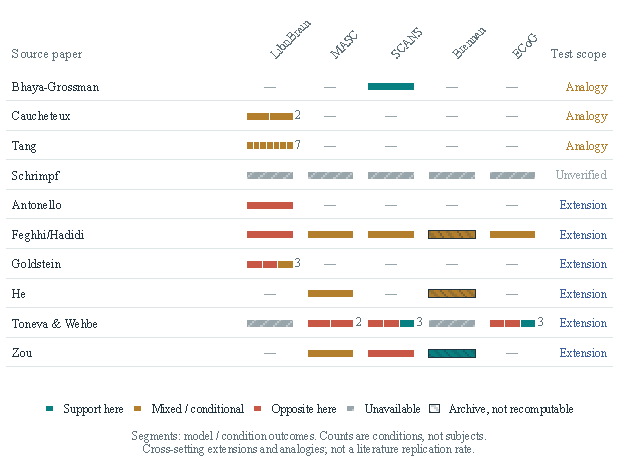
\includegraphics[width=1.0000\textwidth]{../figures_v2/revision_r1_20261007/fig09_scorecard_r1.pdf}
\caption{\textbf{Cross-setting tests and source coverage.} The right column follows scorecard\_transport.tsv: these tests are conceptual extensions or analogies, not literal replications. Each mini-bar displays the stored per-model/condition outcomes for that cohort in scorecard\_derived.json. Colors describe support, conditional/mixed behavior, or the opposite direction under this benchmark's operationalization, not verdicts on the original papers. Numbers count conditions, not independent subjects. Dashes mean no stored entry; hatched gray denotes unavailable evidence. The Schrimpf comparison remains unverified because tensors are missing. Dark-hatched outlined cells read the $49$-listener Brennan archive, which cannot be recomputed (Appendix~\ref{app:brennan}): the Zou cell is not reproduced on the recomputable $47$-listener rebuild, although the same rule still reads ``supports'' there (BERT $36/47$, epochs without a baseline) and its provenance is lost; the Feghhi/Hadidi and He Brennan cells are pending re-derivation. No replication fraction is computed.}
\label{fig:scorecard}
\end{figure}

\newpage

\paragraph{Evidence status.} Nine analyses have executable output-to-outcome mappings; the
baseline comparison does not. Its per-model LibriBrain tensors are missing, and the surviving
GPT-2 maximum is selected over cells where both GPT-2 and BERT passed a threshold, while GloVe's
maximum is unconstrained. That asymmetry favors the baseline, so the reported tie is historical
and unverified. It does not enter a replication tally. Other mappings also changed during audit:
the lag test is an analogue of forecasting, the layer-split result is a between-model contrast,
and the decoding result concerns retrieval rather than continuous reconstruction. These changes
are retained in the provenance files. In particular, the multilingual layer-depth crossover is
an analogy on one cohort, not a replication of the original within-STG physiological contrast.

\paragraph{Brennan lineage.}\label{app:brennan} Two Brennan substrates exist. Every Brennan number in
the main text and in the concordance appendices comes from the $47$-listener rebuild, which pairs the
distributed FieldTrip signal files with the released event markers. Three cells of
Figure~\ref{fig:scorecard} (the Brennan cells of the Zou, Feghhi/Hadidi and He rows) read a
$49$-listener archive built from another release of the recordings (BrainVision files) whose neural
data and preprocessing recipe can no longer be recovered, so these cells cannot be recomputed; we keep
them, marked, as historical, and the companion boundary analysis likewise keeps that archive in an
appendix only. The Zou cell is not reproduced on the recomputable rebuild: a registered re-extraction
on the $47$ listeners gives model means $3$--$8$ times the archive's and a significantly positive
GPT-2-medium; the same scorecard rule (BERT mean above zero, $p<0.05$) still reads ``supports'' there
(BERT $36$ of $47$ listeners, Wilcoxon $p = 1.3\times10^{-5}$), a positive result the companion
analysis attributes to bidirectional right context, the reading-rule question of
Appendix~\ref{app:readrule}; the cell's provenance, not its label, is what is lost. The Feghhi/Hadidi
and He Brennan cells are pending re-derivation on the rebuild. Per listener the two substrates barely
agree (Spearman correlation of the BERT boundary contrast over the $47$ shared listeners $+0.18$) and
we have not identified why. A segment-indexing defect of the first rebuild is excluded as the cause by
the code: that builder drops every listener with fewer than $12$ segment markers, and the archive's
builder maps segments by label. One observation is unexplained: the nine listeners whose recordings
lack the first segment marker have an archived BERT contrast of $-1.5$ against $+13.7\times10^{-3}$
for the other $38$ shared listeners (rebuild $+30.7$ against $+33.8$). The rebuild's alignment of
signal to word markers is verified on one listener (S01) only: a per-listener lag-scan check with
planted offsets, registered after submission, failed its positive control on that listener, also
after a registered $0.5$~Hz high-pass, so it could not certify the others, and an independent check
with another statistic failed the same control (\texttt{PREREG\_paperA\_rebuttal\_checks\_20261004.md},
\S2; receipts in \texttt{paperA\_rebuttal\_20261004/brennan\_align\_raw/}). This caveat applies to every Brennan
number. The lineage comparisons above (the $3$--$8\times$ ratio, BERT $36$ of $47$, the $+0.18$
correlation and the nine-listener split) used the rebuild's epochs as stored, without a baseline, and
were not recomputed after the correction below.

\paragraph{Brennan preprocessing (found after submission).}\label{app:brennan-preproc} The rebuild's
epochs are raw FieldTrip slices: no filter, no baseline, no re-reference, whereas the LibriBrain and
MEG-MASC epochs are baseline-corrected and the fixed-depth route applies no broadband filter
(Appendix~\ref{app:protocol}). Correlation distance removes a per-trial scalar offset, not a
per-channel drift. A registered check, written before any code
(\texttt{PREREG\_paperA\_brennan\_preproc\_20261009.md}; receipts
\texttt{paperA\_rebuttal\_20261004/\allowbreak brennan\_\{preproc,k2\}\_summary\_20261009.json}),
recomputed the Brennan numbers under a per-epoch baseline ($-100$ to $0$~ms; primary) and a linear
detrend over the epoch (secondary). Neither is clean (the baseline window holds the previous word's
response; the detrend line is fit over the response window), so both are reported. On the stored
epochs the per-channel window means carry over $99.99\%$ of each pattern's variance (median), and the
neural dissimilarities correlate with story-time distance (median Spearman $+0.885$, positive in all
$47$ listeners); a baseline or detrend removes this ($+0.002$, $0.000$), while model dissimilarities
barely track story time (median $+0.009$). By the registered rule the drift mechanism is supported. The
similarity ranking of the $32$ checkpoints then correlates $-0.05$ (baseline) and $+0.25$ (detrend)
with the stored one, so the concordance was recomputed in full, encoding target included. With a
baseline (detrended in parentheses; stored epochs after the semicolon): concordance $-0.248$,
checkpoint interval $[-0.55, +0.11]$, family-clustered $[-0.62, +0.14]$ (upper bound $+0.12$ to
$+0.14$ over seeds $0$--$19$) ($-0.047$, $[-0.39, +0.31]$, $[-0.53, +0.39]$), not determined by the
registered reading; split-half ranking reliability $0.45$ for similarity and $0.59$ for encoding
($0.25$, $0.78$; $0.977$, $0.970$); unit-half Kendall $\tau$ $0.64$--$0.70$ with spread
$0.86$--$1.10\times$ the paired-difference SE ($0.58$--$0.75$, $0.82$--$1.52\times$; $0.93$--$0.97$,
$2.4$--$6.8\times$), with the family-level encoding ranking not identifiable (detrended, neither
similarity ranking is either); class gap $+15.6$ ranks, family-clustered $p=0.012$ ($+15.4$,
$p=0.009$; $-0.4$, $p=0.53$), the sign LibriBrain has; word-level RDM reliability $0.677$ ($0.743$;
$0.858$). These use the cached features of the three unspaced checkpoints (their re-extracted
Brennan features were not kept), so the comparable stored concordance is $+0.342$, not $+0.366$. The
eight-segment reliabilities and repeat removal were rerun with the baseline only
(Appendices~\ref{sec:partition},~\ref{app:refuted}). The per-band reliability of
Appendix~\ref{sec:broadband} band-pass filters every band (lowest edge $1$~Hz) and was not rerun.

\section{Narrative Identity versus Finite Word Sampling}\label{sec:partition}

\paragraph{Why the registered primary and co-primary disagree.} The registered primary of ADR 0005
was the variance of the leaderboard across the four stories over its variance under participant
resampling, with confirmation requiring all three criteria jointly; it came out $0.80$
(similarity) and $0.16$ (encoding) against a threshold of $>2$, so the test was not confirmed and
falsifier F1 fired (\S\ref{sec:stimulus}). Post hoc inspection shows why the co-primary
nonetheless met its criterion: all four story-specific rankings are displaced from the pooled
ranking by a similar amount ($\tau = 0.29$--$0.44$, against $0.87$ for a participant resample), so
they are uniformly far from it rather than dispersed around one another, and a variance ratio
cannot see a uniform displacement. That explanation is post hoc --- the failure mode was not
registered --- so it cannot restore confirmatory status. A confirmatory version requires a new
registration with a statistic sensitive to displacement, on a new stimulus set.

\paragraph{Numbers behind Section~\ref{sec:stimulus}.} At full length each story's similarity
leaderboard has Spearman--Brown split-half reliability $0.933$--$0.958$, and the six between-story
agreements have median $-0.411$ and mean $-0.025$. Capped at the shortest story (F4) they have
median $-0.146$ and mean $+0.003$, and The Black Willow's reliability falls to $0.47$. On eight
Brennan segments of about $8\,000$ words, the stored epochs gave similarity (Spearman--Brown)
reliability $0.995$--$0.999$ with encoding undetermined on seven, which we had read as encoding needing
more data than similarity. With a per-epoch baseline (Appendix~\ref{app:brennan-preproc}) similarity
reliability is $0.30$--$0.91$, similarity and encoding are each determined on five segments and both
on four, so that reading does not survive.

Words and narratives vary together above, so a further split separates them. Each story is divided
into two equal, disjoint word partitions, giving eight leaderboards in which a within-story pair
shares the narrative and differs in words, while a between-story pair differs in both, at matched
size throughout.

The two readouts behave differently. Similarity leaderboards from the same story agree at
$+0.556$ on average and from different stories at $-0.008$, a difference of $+0.564$
($95\%$ CI $[+0.35, +0.78]$, one-sided $p = 0.012$): a suggestive within-story advantage that does not establish a narrative-identity mechanism,
given the failed rankability condition below. Encoding shows no such effect --- $+0.509$ within against
$+0.476$ between, difference $+0.034$, CI $[-0.03, +0.09]$ --- so encoding rankings generalize
across narratives about as well as they generalize across disjoint halves of one.

\textbf{This analysis does not meet our pre-registered rankability precondition and is reported as
suggestive}: at $\approx 16\,000$ word-trials per partition only one of eight partitions has both leaderboards
individually determined. Two things argue the signal is real anyway --- within- and between-story
pairs use the \emph{same} partitions with the same reliabilities, so attenuation would shrink both
rather than open a gap, and within-story agreement tracks partition reliability in the direction
attenuation predicts ($0.86/0.64 \to +0.74$ against $0.14/0.32 \to +0.36$). Settling it needs
longer narratives than this cohort provides.

\section{Numerical Failure Modes and Their Detection}\label{app:fragility}

This appendix reports in full the computational failures summarized in \S\ref{sec:fragility}.
All four share one cause: code written as though its inputs were on a unit scale, applied to
neural data stored in physical units, and all four produced plausible numbers rather than errors.

\paragraph{Channel-type metadata.} Trusted channel-type metadata let $14$ EKG and DC channels
carrying $99.97\%$ of total variance into an intracranial analysis, making the result a property
of the stimulus audio track rather than of cortex. Caught by a per-channel variance audit, and
fixed by validating channel types against the recording's own variance profile.

\paragraph{Ridge grid against a rebuilt archive.} A fixed ridge grid met a rebuilt archive at
$\mathrm{std} \approx 10^{-13}$ and returned encoding correlations of exactly $0.00000$ for all
$32$ models --- diagnostic enough to catch on inspection, unlike the third failure.

\paragraph{A guard constant in the correlation denominator.} A $10^{-12}$ guard in a correlation
denominator: at $\mathrm{std} = 3.95\times10^{-7}$ the denominator is of order $10^{-11}$--$10^{-10}$,
and the guard sits beside the variance of \emph{that model's own} predictions, so a
stronger-predicting model is shrunk less. It reordered models scoring between $+0.029$ and
$+0.051$, inflating the readout concordance of an earlier analysis in this project from
$-0.573$ to $-0.678$; changing only that constant recovers $-0.573$, matching an independent
scale-invariant fix to sixteen significant figures. The claim-reproduction harness read $97/97$
green before and after (the registry has since grown to $198$ claims), because it checks stored results against the paper's claims and cannot
see how the results were produced.

\paragraph{Encoding-target scale across LibriBrain sessions (found after submission).} Sessions $9$
and $3$ of the encoding target differ in scale ($76.6\times$ and $5.5\times$ the median session; the
other ten lie within $0.79$--$1.27\times$) and the target was scaled once across sessions, so session
$9$'s rows set the penalty chosen in the folds that contain it. After the single scaling the other
sessions' targets sit far below the unit variance the ridge grid assumes; the grid ceiling 1e6 is
selected in $352$ of $384$ checkpoint-folds (Appendix~\ref{sec:scorecard}) and every encoding score is
lowered, by $1.7$--$3.1\times$ (mean over the $32$ checkpoints $0.102$ with each session scaled
separately against $0.046$ as published). With each session scaled separately the concordance is
$\rho = -0.543$, family-clustered CI $[-0.71, -0.22]$ (branch A in $20$ of $20$ bootstrap seeds); the
reversal does not depend on it, no fold selects the ceiling, and $11$ of $12$ sessions still reverse
on their own. The diagnostic and the re-score were registered after submission and before either ran
(\texttt{PREREG\_paperA\_rebuttal\_checks\_20261004.md}),
with planted rescalings that the diagnostic recovered exactly; the rescaled arm reproduces every
published per-session value when the scaling is switched off. The absolute encoding magnitudes in this
paper (for example class means near $0.05$) are those of the single scaling. In session $9$ the encoding
score stays near zero after rescaling while similarity is ordinary; we have not identified why. The
same defect reaches the Qwen2.5 ladder (Appendix~\ref{sec:scorecard}).

\paragraph{What the bundle holds.} The original artifact, the corrected one, and the isolation
experiment that changes only the guard constant, with harness checks that pin all three values.
These are stored-value checks: the harness does not yet include a test that rescales the neural
data, which is what would detect this failure class before it produces a number; the per-session
scale diagnostic above, with its planted rescalings, is shipped beside it but is not part of the harness.

\section{Geometry Sensitivity and Unresolved Explanations}\label{app:mechanism}

Section~\ref{sec:concordance} established that the reversal is a class-level offset (removing the
architecture-class means leaves a within-class concordance of $-0.25$, n.s., and the
encoding-minus-similarity rank gap separates causal models from the rest by $+25.7$ ranks,
family-clustered two-sided $p = 0.005$), and that standardizing the features attenuates it to a residual
whose family-clustered CI crosses zero. With width matched, the gap stays $+14.1$ ranks over $22$
checkpoints (family-clustered two-sided $p=0.018$); on Brennan EEG the class gap is $+15.6$ ranks
with a per-epoch baseline (family-clustered $p=0.012$; detrended $+15.4$, $p=0.009$), LibriBrain's sign,
against $-0.4$ ($p=0.53$) on the stored epochs, which had no baseline (Appendix~\ref{app:brennan-preproc};
all three with the three unspaced checkpoints' cached features). This appendix reports the candidate mechanism we tested and
could not support, since a benchmark paper should be as explicit about a failed explanation as
about a confirmed one.

\paragraph{RSA-only sensitivity, not an encoding-invariance test.}
We transformed the embeddings of ten models by either adding a random sample-varying rank-one
component or rescaling coordinates. The resulting similarity ranking changes: its correlation
with the original ranking falls to $0.49$ at the largest rogue dose, and to $0.76$ under
coordinate rescaling. The historical analysis correlated these new RSA scores with a
\emph{frozen}, previously computed encoding ranking, obtaining $-0.37$ to $-0.49$ around
$-0.43$ (\texttt{invariance\_intervention.json}). It did not refit encoding after intervention;
these are historical RSA-only sensitivity numbers, not evidence of encoding invariance.

The claimed invariance behind that design was wrong for the rogue arm. Train-fold standardization
removes coordinate scale changes, but adding $s a v^\top$, where $a$ varies across samples,
changes the standardized design. We therefore ran a separate \emph{post hoc} primary-cell diagnostic:
the same ten models, $30{,}000$ shared words, $12$ LibriBrain sessions, depth $0.5$, and the
original outer-session ridge protocol, with both RSA and encoding actually recomputed at raw,
center-only, and centered-plus-rank-one doses $0.3/0.7$. All ten raw baselines replay their
stored per-session scores within $1.1\times10^{-16}$. Centering alone changes RSA order
($\rho=0.927$ vs.\ raw) but leaves encoding scores unchanged to $2.1\times10^{-17}$ and
encoding ranks identical. After rank-one injection, encoding rank correlation with raw falls
to $0.406/0.442$ (largest score shifts $0.0189/0.0255$); the standardized-ridge invariance
premise is falsified on real data (Table~\ref{tab:rogue-ranks}).

\begin{table}[t]
\centering\footnotesize
\caption{\textbf{Post hoc rank-one sensitivity, both readouts recomputed on the same ten models.}
Cells are RSA/encoding ranks (rank 1 = highest) at the fixed LibriBrain primary cell.
Center-only is $X-X_{\mathrm{mean}}$; doses $0.3/0.7$ add a sample-varying rank-one term to that
centered matrix. The old frozen-encoding RSA-only injection is not mixed into these ranks.}
\label{tab:rogue-ranks}
\begin{tabular}{lrrrr}
\toprule
Model & Raw & Center only & Rogue $0.3$ & Rogue $0.7$ \\
\midrule
Pythia-70M     & 7/2  & 6/2  & 6/1  & 5/1 \\
Pythia-160M    & 5/3  & 7/3  & 7/8  & 7/8 \\
Pythia-410M    & 9/1  & 9/1  & 9/7  & 9/7 \\
GPT-2          & 8/8  & 8/8  & 10/5 & 10/6 \\
GPT-2-medium   & 10/6 & 10/6 & 8/2  & 8/2 \\
BERT-base      & 4/7  & 5/7  & 5/4  & 6/4 \\
BERT-large     & 6/9  & 4/9  & 4/9  & 4/9 \\
RoBERTa-base   & 3/4  & 3/4  & 3/3  & 3/3 \\
T5-base        & 2/10 & 1/10 & 2/10 & 1/10 \\
T5-large       & 1/5  & 2/5  & 1/6  & 2/5 \\
\bottomrule
\end{tabular}
\end{table}

The RSA--encoding rank concordance changes from $-0.261$ raw to $-0.406$ centered and
$-0.248/-0.164$ after the two added-direction doses. Five-family block-bootstrap intervals
for the encoding-rank correlations at doses $0.3/0.7$ are wide
($[-0.098,1.000]$/$[-0.105,1.000]$); the ten models do not identify a general mechanism.
The perturbation is synthetic and is not the models' endogenous anisotropy. Thus actual
encoding movement overturns the old invariance premise, but neither proves that anisotropy
causes the original cross-readout disagreement nor excludes other geometry explanations.

\paragraph{Anisotropy.} Cosine-distance RSA is sensitive to a dominant mean/rogue direction, while
ridge encoding standardizes its inputs. Autoregressive models are extremely anisotropic: the median
causal model has participation ratio $1.0$, its top principal component alone explaining
$\approx 98\%$ of feature variance, the known anisotropy and ``rogue dimension'' phenomenon of
transformer language models, most extreme in autoregressive ones \citep{ethayarajh2019contextual,
timkey2021rogue, gao2019degeneration}; masked and
encoder--decoder models are near-isotropic (participation ratio $164$ and $95$). Standardizing each
model's features before RSA removes that dominance and attenuates the reversal from $-0.573$ to
$-0.479$ (mean-centered) to $-0.432$ (per-dimension standardized), while encoding is unchanged. We do
not read the remainder as a readout-operation residual: the standardized residual's
family-clustered CI crosses zero ($[-0.73, +0.23]$), and the new random-direction
intervention cannot identify which naturally occurring geometry causes the original reversal.
Even standardized, causal models keep the lower RSA and higher encoding (RSA $0.006$ versus
masked $0.007$ versus enc--dec $0.009$; encoding $0.049$ versus $0.041$ versus $0.043$), which describes a remaining point-estimate difference, not an identified mechanism: RSA rewards
representations whose dominant geometry matches the brain, encoding rewards representations linearly
concentrated onto the neural response, and the anisotropy that separates autoregressive from
bidirectional models sits on opposite sides of that trade-off. A principal-component truncation
makes the same point descriptively (Figure~\ref{fig:mechanism}a): encoding peaks at the top few
components and then falls, while similarity keeps rising as more of the dominant geometry is added.

\begin{figure}[t]
\centering
\includegraphics[width=1.0000\textwidth]{../figures_v2/integrated_20260923/fig10_redrawn.pdf}
\caption{\textbf{Effective dimensionality covaries with the readout gap.} (a) Architecture-averaged PCA-truncation curves, shown as an illustrative diagnostic; solid is encoding, dashed RSA. (b) Participation ratio against the corrected primary-score gap for all 32 checkpoints. The within-autoregressive relation (rho=-0.76, n=18 in six families) is highlighted; the pooled rho=-0.65 is not interpreted causally or as 32 independent models. Family-clustered intervals and the between-class decomposition remain in the text. Sources: pctrunc receipts and concordance32\_CORRECTED.json.}
\label{fig:mechanism}
\end{figure}

\paragraph{Exploratory association within the autoregressive class.} Pooled over all 32 checkpoints
participation ratio correlates with the encoding$-$RSA gap ($\rho = -0.65$, family-clustered $95\%$
CI $[-0.87, -0.02]$). That interval excludes zero only barely, and the pooled number carries the
same between-class inflation as the reversal itself (whose within-class concordance is
$\rho = -0.25$, $p = 0.16$), so pooled it is close to a restatement of ``is it causal''. The test that is not is
available inside the one class where participation ratio actually varies. Among the $18$
autoregressive checkpoints, over $6$ families, the more anisotropic models show the larger readout
gap ($\rho = -0.76$, family-clustered $95\%$ CI $[-0.93, -0.09]$ excluding zero; leaving out any
single family moves it only within $[-0.85, -0.66]$). Inside the masked and encoder--decoder classes
the relation is absent ($+0.07$ and $+0.10$, both n.s.), as expected where participation ratio is
near-ceiling. What we cannot claim
is a single mechanism spanning all three classes: the pooled correlation survives clustering only
marginally and is mostly the between-class offset, so it does not establish a relation that holds
\emph{within} each class. Our pre-registered prediction, that brain-relevant signal sits in
\emph{non-dominant} components, was not supported; this effective-dimensionality account is
exploratory. Table~\ref{tab:decomp} collects the decomposition and the per-class mechanism.

\begin{table}[t]
\centering
\small
\caption{Where the readout gap lives, and where dimensionality covaries with it. \emph{Top:} the overall rank
correlation is carried by a between-class offset. \emph{Bottom:} per class. Similarity ranks the
classes encoder--decoder $>$ masked $>$ causal while encoding ranks them causal $>$
encoder--decoder $>$ masked, which is the whole reversal; the ENC$-$RSA rank gap separates causal
from the rest ($+25.7$ ranks, family-clustered two-sided $p = 0.005$). Participation ratio predicts that gap
\emph{inside} the causal class, where it varies, with a family-clustered CI excluding zero; inside
the other two classes participation ratio is near-ceiling and the relation is absent. CIs resample
model families, not checkpoints; the masked and encoder--decoder classes contain only four and two
families, too few for a stable clustered CI, so their point estimates are given without one.}
\label{tab:decomp}
\begin{tabular}{@{}lrrrrrr@{}}
\toprule
\multicolumn{7}{@{}l}{\emph{Concordance decomposition (32 checkpoints, 12 families, 3 classes)}}\\
\midrule
\multicolumn{5}{@{}l}{overall similarity-vs-encoding concordance} & $\rho = -0.573$ & $p = 6\times10^{-4}$\\
\multicolumn{5}{@{}l}{after removing architecture-class means} & $\rho = -0.25$ & $p = 0.16$\\
\multicolumn{5}{@{}l}{between-class share of $|\rho|$} & $56\%$ & \\
\midrule
\multicolumn{7}{@{}l}{\emph{Per architecture class}}\\
\midrule
class & $n$ & fam. & mean RSA & mean ENC & rank gap & PR--gap $\rho$ [family CI]\\
\midrule
causal          & $18$ & $6$ & $0.0049$ & $0.0494$ & $+11.2$ & $-0.76$ $[-0.93, -0.09]$\\
encoder--decoder & $5$ & $2$ & $0.0101$ & $0.0426$ & $-18.8$ & $+0.10$ (CI unstable)\\
masked          &  $9$ & $4$ & $0.0082$ & $0.0412$ & $-12.0$ & $+0.07$ (CI unstable)\\
\bottomrule
\end{tabular}
\end{table}

\paragraph{A learned encoder does not resolve it, and why.} If the disagreement were an artifact of
hand-crafted neural features, a powerful learned encoder should reconcile the two readouts. We
trained a diagonal state-space (S4D) encoder on the raw word-locked MEG with a self-supervised
masked-reconstruction objective (no language model involved) and used its 128-dimensional embedding
as both readouts' neural representation. The concordance collapses to $\rho_z = +0.07$ (n.s.;
$\rho_z$ is the headline concordance statistic recomputed with the learned embedding $z$ in place
of the raw neural pattern). This
is \emph{not} evidence that the reversal was a featurization artifact. A diagnostic shows the
learned embedding's word dissimilarity matrix is near-degenerate (pairwise-distance standard
deviation $0.005$ versus $0.23$ for the raw pattern) and uncorrelated with the raw neural RDM
($\rho \approx 0.01$): reconstruction pre-training captured the word-\emph{general} evoked response
and discarded word-\emph{discriminative} geometry, so both readouts lose their ability to rank
models (RSA ranking reliability falls $0.98 \to 0.61$). The test is therefore uninformative rather
than a refutation, and it carries a caution of its own: reconstruction-trained neural encoders can
flatten exactly the fine word-level structure that RSA-based brain--model alignment depends on.

\section{Leaderboard Reliability in ML}\label{app:related-ml}

The instabilities we measure have direct ML analogues: benchmark conclusions can depend on the
arbitrary composition of the suite \citep{dehghani2021benchmark}, small evaluation sets leave
model comparisons underpowered \citep{card2020little}, and evaluation frameworks respond by
making coverage and uncertainty explicit \citep{liang2023holistic} or by collecting evaluation data
dynamically \citep{kiela2021dynabench}.
Brain--LLM benchmarks add a variance axis those suites lack: participants and stimuli are
\emph{both} samples, and \S\ref{sec:stimulus} shows the conclusion can change depending on
which one the error bar resamples.

\section*{Documentation, Hosting, Licensing, and Maintenance}\label{availability}

\textbf{What will be released.} On publication, the BrainLLM-Bench release will have two parts: (i) the
fixed protocol as a runnable harness (band-splitting, regioning, RSA,
confound battery, per-band ceilings, clustered nulls) with a datasheet
documenting each cohort's provenance, size, and preprocessing; and (ii) the
precomputed alignment tensors, the per-cohort headline cells for the four fully controlled
cohorts, and the scorecard, so a new model can be ranked without recomputing the existing entries.
A subset is released at \coderepo: the harness, its
stored-result checks, the datasheet, the derived result files and the sensor-region atlases.
The missing baseline tensors and raw-data rerun requirements are disclosed above; public hosting
and deposition remain as described below.

\textbf{Access and licensing.} The harness will be released under a permissive open-source
license; derived tensors and tables will be released under the terms of the recordings they are
computed from, so those derived from LibriBrain (CC BY-NC 4.0) are non-commercial. The underlying
recordings keep their original licenses and are obtained from source: LibriBrain (CC BY-NC 4.0),
MEG-MASC (CC0), MEG-SCANS (OpenNeuro \texttt{ds006468}, CC0) and the ``Podcast'' ECoG
dataset (OpenNeuro \texttt{ds005574}, CC0) are public, the Brennan EEG cohort is distributed by
its authors through a university data repository under CC BY 4.0, per its DataCite record \citep{brennan2018alice}, and the fMRI cohort
ds003020 is on OpenNeuro (CC0) \citep{lebel2026openneuro}. We will redistribute derived word
lists, region maps and alignment tensors, not raw recordings, following each source's
redistribution and attribution terms.

\textbf{Hosting and maintenance (release plan).} On publication, the code and
precomputed tensors will be hosted in a public version-controlled repository with a
tagged release matching this paper, and that release will additionally be deposited
in a persistent archive with a citable DOI (Zenodo), so the artifact remains
resolvable independent of the code host. The datasheet, leaderboard, and scorecard will be versioned alongside the
code under semantic versioning, so every reported number is pinned to both a commit
and a release tag, and the precomputed tensors will ship with standardized dataset
metadata (Croissant) for machine-readable discovery. New models and cohorts are
intended to enter through the harness of Section~\ref{sec:harness}: a submission runs
the fixed protocol, emits the same tensor schema, and is added to the leaderboard
through a versioned pull-request review that checks protocol conformance before
merge, so growth does not silently change the scoring. The leaderboard and scorecard
are the intended points of community growth, and the review checklist and issue
tracker will be public so that maintenance is not tied to a single person.

\begin{table}[t]
\centering
\setlength{\tabcolsep}{4pt}
\begin{tabular}{lllrr}
\toprule
Cohort & Modality & Language & Recordings & Subjects/patients \\
\midrule
LibriBrain \citep{ozdogan2025libribrain} & MEG & English & 36 & 1 \\
MEG-MASC \citep{gwilliams2023megmasc} & MEG & English & 76 & 10 (27 rebuilt) \\
MEG-SCANS \citep{habersetzer2025megscans} & MEG & German & 92 & 23 (of 24) \\
Brennan \citep{brennan2019hierarchical} & EEG & English & n/a & 49 (47 analysed) \\
ECoG ds005574 \citep{zada2025podcast} & ECoG & English & n/a & 9 \\
\bottomrule
\end{tabular}
\caption{The five benchmark cohorts. Modality spans MEG, scalp EEG, and
intracranial ECoG; language spans English and German. The task is natural
language comprehension throughout.}
\label{tab:cohorts}
\end{table}

\section*{Datasheet (Summary)}\label{datasheet}

Following the datasheet structure of \citet{gebru2021datasheets}, the release
documents each cohort along the standard axes; a condensed form appears in
Table~\ref{tab:datasheet}. \emph{Motivation}: to make brain--LLM alignment results
comparable under one protocol. \emph{Composition}: five cohorts, per-word neural
response patterns crossed with per-layer model features, with lexical confounds and
reliability ceilings attached. \emph{Collection}: inherited from each source
dataset's published acquisition. \emph{Preprocessing}: the fixed protocol of
Section~\ref{sec:tensor} (band-splitting, regioning, RSA, confound
partialization, per-band ceilings, clustered nulls). \emph{Uses}: benchmarking new
models and cohorts, auditing prior claims. \emph{Distribution and maintenance}: as
in the documentation, hosting, licensing, and maintenance section above, under
an open-source license (code) and each source's terms (derived tensors;
non-commercial for LibriBrain), versioned to this paper's release.

\begin{table}[t]
\centering
\small
\begin{tabular}{lllrr}
\toprule
Cohort & Modality & Language & Subjects & Sensors \\
\midrule
LibriBrain & MEG & English & 1 (12 sessions; 36 recordings) & 306 \\
MEG-MASC & MEG & English & 10\textsuperscript{b} & 208 \\
MEG-SCANS & MEG & German & 23 & 306 \\
Brennan & EEG & English & 49 (47 analysed)\textsuperscript{d} & 60\textsuperscript{c} \\
ECoG (ds005574) & intracranial & English & 9 & grid (MNI ROIs) \\
\bottomrule
\end{tabular}
\caption{Datasheet summary of the five cohorts. Four (LibriBrain, MEG-MASC,
MEG-SCANS, ECoG) are scored under the full confound-controlled RSA protocol; the
Brennan EEG cohort enters the scorecard and the fixed-depth readout comparison.
\textsuperscript{b}The tensor build uses the 10-subject preprocessed archive; the
stimulus-generalization and concordance analyses (\S\ref{sec:stimulus}, \S\ref{sec:concordance})
use the full 27-subject cohort rebuilt from raw, and the text names which build each result uses.
\textsuperscript{c}61-electrode cap; 60 channels enter the stored epochs and every analysis.
\textsuperscript{d}Every Brennan computation in the main text uses the $47$-listener rebuild (two
listeners' public files are corrupt); only three scorecard cells read the $49$-listener archive
(Appendix~\ref{app:brennan}).}
\label{tab:datasheet}
\end{table}


\section*{Historical Scorecard: Operationalizations and Legacy Labels}\label{app:scorecard-detail}

Table~\ref{tab:scorecard-detail} expands each row of the ten-claim scorecard
(\S\ref{sec:scorecard}, Table~\ref{tab:scorecard}) into the operationalization the
benchmark ran, its results and original labels. These legacy labels are retained for provenance;
Table~\ref{tab:scorecard} gives the current scoped outcomes. They do not imply direct replication.

\begin{longtable}{@{}p{2.1cm} p{3.8cm} p{5.1cm} p{1.5cm}@{}}
\caption{Historical scorecard detail: tested operationalizations, stored results and legacy labels. Current scoped outcomes and missing-data status are in Table~\ref{tab:scorecard}; legacy labels are not replication verdicts (\S\ref{sec:scorecard}). The stored operationalization strings (``7-LLM'', ``5-cohort'') predate the counts used here, which follow the receipts (six tensor-route LLMs; four boundary cohorts).}\label{tab:scorecard-detail}\\
\toprule
Prior claim (venue) & Benchmark operationalization & Result & Legacy label \\
\midrule \endfirsthead
\multicolumn{4}{c}{\tablename\ \thetable\ (continued)}\\ \toprule Prior claim (venue) & Benchmark operationalization & Result & Legacy label \\ \midrule \endhead
\midrule \multicolumn{4}{r}{\footnotesize continued on next page}\\ \endfoot
\bottomrule \endlastfoot
Tang et al. (Nat. Neurosci.) & Trial-level contrastive retrieval LLM $\gets$ MEG on the LibriBrain headline cell (superseding a naive ridge decoder that had read as null, $R^2 = -0.004$). & Refines: a weaker relative transfers --- retrieval clears chance on all seven targets (six models, GPT-2 at two segmentations; $5.7$--$6.5\times$ at top-10; shuffled-target $0.7\times$) while absolute accuracy stays far below continuous reconstruction (top-1 $0.03\%$, median rank $2143$ of $9495$). Modality, temporal-resolution and task-family boundary added: theirs is open-ended generation, ours closed-set retrieval, the contrast their own abstract draws. & refine \\ \addlinespace
Toneva \& Wehbe (NeurIPS) & Per-(region, LLM, layer) headline-cell scan across 5 cohorts with the six tensor-route LLMs. & Their claim as stated --- middle layers beating both shallower and deeper --- holds in $2$ of the $8$ recomputable cells; the weaker reading (mid-to-shallow over deep) holds on the 3 MEG cohorts: mid-to-shallow LLM layers carry the headline cell on LibriBrain, MEG-MASC and MEG-SCANS (Brennan has no headline cell under the tensor protocol), though the peak latency is cohort-specific ($\approx$346 ms on LibriBrain, 467--768 ms on MEG-MASC, 527--587 ms on MEG-SCANS). ECoG refines the picture: deep layers win on the ECoG headline cell, so the mid-layer story is conditional; their own Fig.~4 offers context length as a competing account of that flip (their deepest layers peak below ten words of context, ours is sentence context). & refine \\ \addlinespace
Schrimpf et al. (PNAS) & Cross-cohort headline z(rho) for the tensor-route LLMs vs random + GloVe + phonemic baselines (LibriBrain, MEG-MASC, MEG-SCANS, Brennan, ECoG). & Replicates qualitatively: LLMs $\gg$ random (historical noise floor, not recomputable), contextual > GloVe in cell-count breadth + layer-depth gradient. But GloVe-300 ties GPT-2 on raw headline magnitude (6.7 vs 6.1, $\times 10^{-3}$; historical, unverified), so the contextual-over-static advantage holds in breadth, not single-cell magnitude; the accuracy--brain-score correlation that is their actual claim is not re-measured here. & refine \\ \addlinespace
Caucheteux et al. (Nat. Hum. Behav.) & Lag analogue of their forecast test (they augment present-word activations with predictions spanning multiple timescales and map onto fMRI in $304$ listeners; we shift the model's word sequence against the brain's on the LibriBrain headline cell and locate the peak shift, per post-onset window). & Anticipation is windowed, not general: GPT-2 peaks $+1$ word ahead only in the 350--550~ms windows, peaks \emph{behind} at 150--250~ms, and peaks at zero lag when collapsed over time; BERT shows no forward peak at any window. & refine \\ \addlinespace
Goldstein et al. (Nat. Commun.) & Their claim: in ECoG high-gamma, layer index tracks peak-encoding lag, strongest in Broca's area, for GPT-2 XL and Llama-2. Our analogue: per-(region, LLM, band) layer $\times$ peak-time Spearman, run on 5 cohorts; stored receipts cover LibriBrain only. Their nine-patient podcast ECoG cohort appears to be the recordings of our ECoG cohort, so an ECoG cell would not change the setting. & Reproduced for BERT temporal\_R (r=+0.73 broadband, +0.82 theta) --- an architecture they did not test --- while the GPT family, their own model class, inverts in the delta band (r=-0.85 to -0.91). Their claim was never stated across frequency bands; adding that dimension, the hierarchy holds neither uniformly across bands nor across architectures. & refine \\ \addlinespace
Zou et al. (Nat. Neurosci.) & 4-cohort $\times$ 6-LLM $\times$ 2-band boundary-conditional RSA; incl. reverse direction with German LLMs. & Consistent with \citet{zou2026constituent} in 7/12 English cells (historical count; the stored cell file gives 5/9; the Brennan cell reads the non-recomputable 49-listener archive, Appendix~\ref{app:brennan}). In German the effect is model-dependent, not uniformly reversed: multilingual BERT reverses significantly (7/23, p=0.005), German-BERT is null (p=0.96) and German-GPT-2 only trends negative (p=0.09), so we record a model-conditional instability rather than a language mechanism. & refine \\ \addlinespace
Bhaya-Grossman et al. (Nature) & Layer-split contrast multilingual-BERT vs German-native LLMs across LLM depths on $6$ subjects of the $23$-subject MEG-SCANS cohort. & Multilingual-BERT wins at shallow layers, German-BERT at deep layers. Their split --- shared acoustic--phonetic encoding versus experience-dependent word-boundary, word-frequency and phonotactic encoding, reported \emph{within the same STG neural populations}, not across regions --- appears here as a split along LLM depth. Cross-modality and cross-language analogue only: their cohort is ECoG in Spanish, English and Mandarin. & \textbf{replicate} \\ \addlinespace
Hadidi et al. (Nat. Commun.) & Their confounds, positional signals and word rate, as a confound-partialling battery (three blocks, then an extended six: word rate, position, length, log frequency, lag-1 MEG components, chronology) per cohort and per subject; their datasets are fMRI and ECoG (reading passages or sentences, and listening to stories), ours MEG listening. & Pooled BERT on LibriBrain retains 47\% under the extended battery (95\% under the first); the pooled GPT family drops to 0\%, but per-subject MEG-MASC GPT-2 retains 36\% in 6/10 subjects. The confound critique applies, but the signal is not removed under per-subject disaggregation. Static word embeddings, the dominant confound for trained models in \citet{lai2025illusions}, are not in this battery. & refine \\ \addlinespace
Antonello et al. (NeurIPS) & Their claim: fMRI encoding performance scales logarithmically with size, $125$M--$30$B, for unidirectional models (OPT, LLaMA). Like-for-like arm: the registered Qwen $0.5$B--$72$B encoding ladder, plus the six-point Pythia $70$M$\to$$2.8$B ladder scored per session at the pre-registered depth; the BERT/GPT-2 RSA comparison is a secondary arm outside their model class. & On the registered bounded-alpha grid, with the rungs re-extracted after the tokenization defect, the ordering reverses on LibriBrain (encoding $\rho=-0.96$; $72$B vs $0.5$B $p=0.0005$), but a post hoc training-fold-expanded grid attenuates the size correlation to $-0.464$ while retaining a $72$B deficit; on MEG-MASC the encoding arm fails its rankability gate and is not determined; under the similarity readout size orders positively ($\rho=+0.93$, $p=0.001$), so the verdict is stated for encoding only. Outside their model class, BERT-base ($110$M, masked) leads at $13.1\times10^{-3}$, above the three-times-larger GPT-2-medium ($355$M, $6.9\times10^{-3}$); across the ladder size does not predict alignment ($\rho = -0.14$, $p = 0.79$) and $2.8$B sits nominally below $70$M at forty times the parameters ($p = 0.23$). In these ladders parameter count did not order alignment. & \textbf{contradict} \\ \addlinespace
He et al. (NeurIPS) & Iterative residual disentanglement (lexicon, syntax, meaning, reasoning; they test one model family) on LibriBrain, then the reasoning residual split medial versus constituent-onset, read out as alignment per model. & The medial-minus-onset contrast of the \emph{reasoning} residual sign-inverts between architectures (LibriBrain: GPT-2 $z=+13.1\times10^{-3}$, BERT $z=-15.7\times10^{-3}$). The \emph{meaning} component also inverts but in the opposite direction and roughly fifteen times smaller (GPT-2 $-0.7$, BERT $+0.9\times10^{-3}$), so the architecture-conditional effect is carried by the boundary term, not the semantic one. & refine \\ \addlinespace
\end{longtable}


\section{Figure and table sources}
\label{app:sources}
Every number in a figure or table is read from a committed receipt in the code release; the files and generators are listed here rather than in the captions.
{\small\begin{longtable}{@{}p{0.13\textwidth}>{\raggedright\arraybackslash}p{0.83\textwidth}@{}}
\toprule Item & Receipts and generator \\ \midrule
\endhead
Fig.~\ref{fig:overview} & Receipts: \texttt{crossed\_narrative/}, \texttt{ds003020/}, \texttt{concordance32\_CORRECTED}, \texttt{concordance\_spacefix\_masc27\_32}, \texttt{brennan\_k2\_summary\_20261009}. \\
Table~\ref{tab:checkpoints} & \texttt{codes/model\_families.py}. \\
Table~\ref{tab:percohort} & Source:
\texttt{results/cross\_cohort\_summary.tsv}. \\
Table~\ref{tab:c4} & Receipts:
\texttt{p4\_encoding/\allowbreak concordance32\_c4.json} (aggregate) and \texttt{p4\_encoding/\allowbreak c4\_static32/}
(one gate-and-score receipt per checkpoint). \\
Table~\ref{tab:ceiling} & Source: \texttt{results/p2\_perband\_ceiling.json}. \\
Fig.~\ref{fig:scorecard} & Drawn by \texttt{codes/fig\_paperA\_scorecard\_r1\_20261007.py}. \\
Table~\ref{tab:rogue-ranks} & Source: \texttt{rogue\_encoding\_20260922/summary.json} and ten four-condition model receipts. \\
Table~\ref{tab:scorecard-detail} & \texttt{results/scorecard/scorecard.tsv}; counts from \texttt{headline\_layer\_scan.tsv} (six tensor-route LLMs) and \texttt{exp\_boundary\_conditional/} (four boundary cohorts). \\
\bottomrule
\end{longtable}}

\end{document}
